% ============================================================
%  MONOGRAPH MASTER FILE
%
%  On the Partition Algebra of Bounded Phase Space:
%  A Unified Framework for Categorical State Counting,
%  High-Energy Trigger Design, and Runtime Verification
%
%  Compile instructions:
%  1. Compile each individual paper to PDF first (see list below).
%  2. Then: pdflatex monograph.tex  (2 passes for correct TOC)
%
%  Individual papers (in order):
%    trajectory-of-upcoming-events.pdf  [Introduction -- already compiled]
%    mathematical-foundation/mathematical-foundation.tex
%    planck-depth-trigger-design/planck-depth-trigger-design.tex
%    high-energy-partition-spectrometer/high-energy-partition-spectrometer.tex
%    multi-subsystem/multi-subystem-qnd-classification.tex
%    angular-resolution/angular-resolution.tex
%    trajectory-completion/trajectory-completion-mechanism.tex
%    fundamental-timing/fundamental-timing.tex
%    virtual-particles/virtual-particles.tex
%    cascade-catalysts/cascade-catalysts.tex
%    comsological-consequences/cosmological-consequences.tex
%    experimental-validation/experimental-validation.tex
%    operating-system/partition-coordinate-refinement/partition-coordinate-refinement-types.tex
%    operating-system/verification-primitive/three-route-verification-primitive.tex
%    operating-system/runtime-primitive/universal-runtime-primitive.tex
%    operating-system/operational-bisimulation/operational-bisimulation-equation-identity.tex
%    operating-system/dispath-substrate/dispatch-substrate-kernel.tex
%    runtime-operations/runtime-operations.tex
% ============================================================

\documentclass[12pt,a4paper,openany]{book}

\usepackage[utf8]{inputenc}
\usepackage[T1]{fontenc}
\usepackage{lmodern}
\usepackage[a4paper,
            top=2.5cm,
            bottom=2.5cm,
            left=2.8cm,
            right=2.8cm]{geometry}
\usepackage{amsmath,amssymb}
\usepackage{microtype}
\usepackage{xcolor}
\usepackage{fancyhdr}
\usepackage{titlesec}
\usepackage{titletoc}
\usepackage{emptypage}
\usepackage{pdfpages}
\usepackage[colorlinks=true,
            linkcolor=blue!50!black,
            citecolor=blue!50!black,
            urlcolor=blue!50!black]{hyperref}

% ---- Page style -------------------------------------------------------
\pagestyle{fancy}
\fancyhf{}
\fancyhead[LE]{\small\nouppercase{\leftmark}}
\fancyhead[RO]{\small\nouppercase{\rightmark}}
\fancyfoot[C]{\thepage}
\renewcommand{\headrulewidth}{0.4pt}

% ---- Chapter/Part style -----------------------------------------------
\titleformat{\part}[display]
  {\normalfont\Huge\bfseries\centering}
  {\partname\ \thepart}{20pt}{\Huge}
\titleformat{\chapter}[display]
  {\normalfont\Large\bfseries}
  {Paper \thechapter}{10pt}{\LARGE}

% ---- TOC depth and style ----------------------------------------------
\setcounter{tocdepth}{1}

% ---- pdfpages setup ---------------------------------------------------
% includepdf options applied globally via \includepdfset
\includepdfset{
  fitpaper=true,
  pagecommand={\thispagestyle{fancy}}
}

% =========================================================
\begin{document}

% ------ Half-title page ------------------------------------------
\thispagestyle{empty}
\vspace*{6cm}
\begin{center}
{\Huge\bfseries On the Partition Algebra of Bounded Phase Space}\\[1.5ex]
{\large A Unified Framework for Categorical State Counting,\\
High-Energy Trigger Design, and Runtime Verification}
\end{center}
\vfill
\clearpage

% ------ Title page -----------------------------------------------
\thispagestyle{empty}
\begin{center}
\vspace*{2cm}
{\Huge\bfseries On the Partition Algebra\\[0.4ex]
of Bounded Phase Space}\\[2ex]
\rule{\textwidth}{1pt}\\[1.5ex]
{\Large A Unified Framework for Categorical State Counting,\\[0.4ex]
High-Energy Trigger Design, and Runtime Verification}\\[3ex]
\rule{\textwidth}{0.5pt}\\[3cm]
{\Large Kundai Farai Sachikonye}\\[1ex]
{\large Technical University of Munich}\\
{\large Chair of Proteomics and Bioanalytics}\\[1cm]
{\normalsize AIMe Registry for Artificial Intelligence}\\[2cm]
{\normalsize \today}
\vfill
\end{center}
\clearpage

% ------ Copyright / note page ------------------------------------
\thispagestyle{empty}
\vspace*{\fill}
\noindent\textit{All papers in this monograph are derived from a single
Bounded Phase Space Axiom. The operating-system framework
(Part~V) and the closed-loop paper (Part~VI) establish the
formal computational substrate over which the partition-physics
derivations are executed at runtime.}
\par\vspace{2ex}
\noindent Each paper in this collection is self-contained and may be compiled
independently. The monograph master file assembles all compiled PDFs into a
single volume. Cross-citations between papers use the \texttt{companion:*}
family of bibtex keys.
\vspace*{\fill}
\clearpage

% ------ Table of contents ----------------------------------------
\tableofcontents
\clearpage

% ------ Preface --------------------------------------------------
\chapter*{Preface}
\addcontentsline{toc}{chapter}{Preface}
\markboth{Preface}{Preface}

This monograph presents a unified framework deriving all principal results
of particle-physics trigger design from a single axiom: that every persistent
physical system occupies a bounded region of phase space with finite Liouville
measure. From this axiom, via the Poincar\'e recurrence theorem and the
algebra of integer partitions, one derives the partition coordinates
$(n, \ell, m, s)$, the shell capacity $C(n) = 2n^2$, the
composition-inflation formula $T(n,d) = d(d+1)^{n-1}$, the Planck depth
$n_P = 60$ for the LHC, and every quantitative design parameter of the
ATLAS real-time event-selection system.

The monograph opens with an \textbf{Introduction} that establishes the
mathematical foundation on which all subsequent results rest: the canonical
bijection $\Phi : \mathbb{Z}^+ \to \mathcal{P}$ from the positive integers
to the partition states of a bounded Hamiltonian system. Three results are
proved: the Partition Bijection ($\Phi$ exists, is unique, and is explicit);
Strict Monotonicity (the partition count $M(t)$ is non-decreasing under any
physical evolution); and the Causal-Partition Uniqueness and Successor
Existence theorems (every state has a unique forward sequence, time reversal
is formally incoherent). These results ground the arrow of time as a
counting theorem rather than a thermodynamic assumption, and establish the
forward sequence $\{M_t, M_t+1, \ldots, M_{\max}\}$ as a finitely
enumerable, bijectively labelled structure.

The monograph is organised in six parts following this introduction.

\textbf{Part~I} (Papers~1--2) establishes the mathematical foundations:
the partition algebra, the Planck depth, and the compositional structure of
the partition state space.

\textbf{Part~II} (Papers~3--5) applies the foundations to measurement:
the LHC as a high-energy partition spectrometer governed by the partition
Lagrangian, the four-subsystem CSCO and QND property, and the angular
resolution of calorimeter detectors as a counting theorem.

\textbf{Part~III} (Papers~6--8) develops trajectory and dynamic analysis:
backward trajectory completion in $\mathcal{O}(\log_3 N)$, the 25~ns
timing window derived from detector geometry, and virtual particles
identified with virtual sub-states.

\textbf{Part~IV} (Papers~9--11) covers algebraic structure and
consequences: cascade catalyst algebra (which coincides with the
renormalisation group), cosmological consequences including the
cosmological constant as partition pressure, and the full experimental
validation programme from keV to TeV.

\textbf{Part~V} (Papers~12--16) presents the operating-system framework:
a refinement-type system over the vaHera AST in which selection rules are
type predicates, three-route equivalence as a verification primitive, a
universal closed-form for transport coefficients subsumng eight classical
formulas, operational bisimulation for cross-framework equation identity,
and the five-subsystem dispatch kernel.

\textbf{Part~VI} (Paper~17) closes the loop: the Tempus trigger program
is compiled to vaHera, dispatched by the kernel, and proved to compute the
same partition classification as the direct physics derivation on every input
event (the Tempus-Physics Bisimulation Theorem).

\vspace{1em}
\noindent The single axiom, the seventeen papers, and the formal bisimulation
together constitute a complete derivation from first principles to running
software.

\vspace{2em}
\noindent\hfill\textit{Kundai Farai Sachikonye}\\
\hfill\textit{Technical University of Munich, \today}

\clearpage

% =================================================================
% INTRODUCTION — THE PARTITION BIJECTION
% =================================================================

% A blank page separates the preface from the introduction.
\clearpage

\phantomsection
\addcontentsline{toc}{chapter}%
  {Introduction --- On the Bijective Correspondence Between Integer
   Sequences and Partition States in Bounded Hamiltonian Systems}

\markboth{Introduction}{On the Bijective Correspondence}

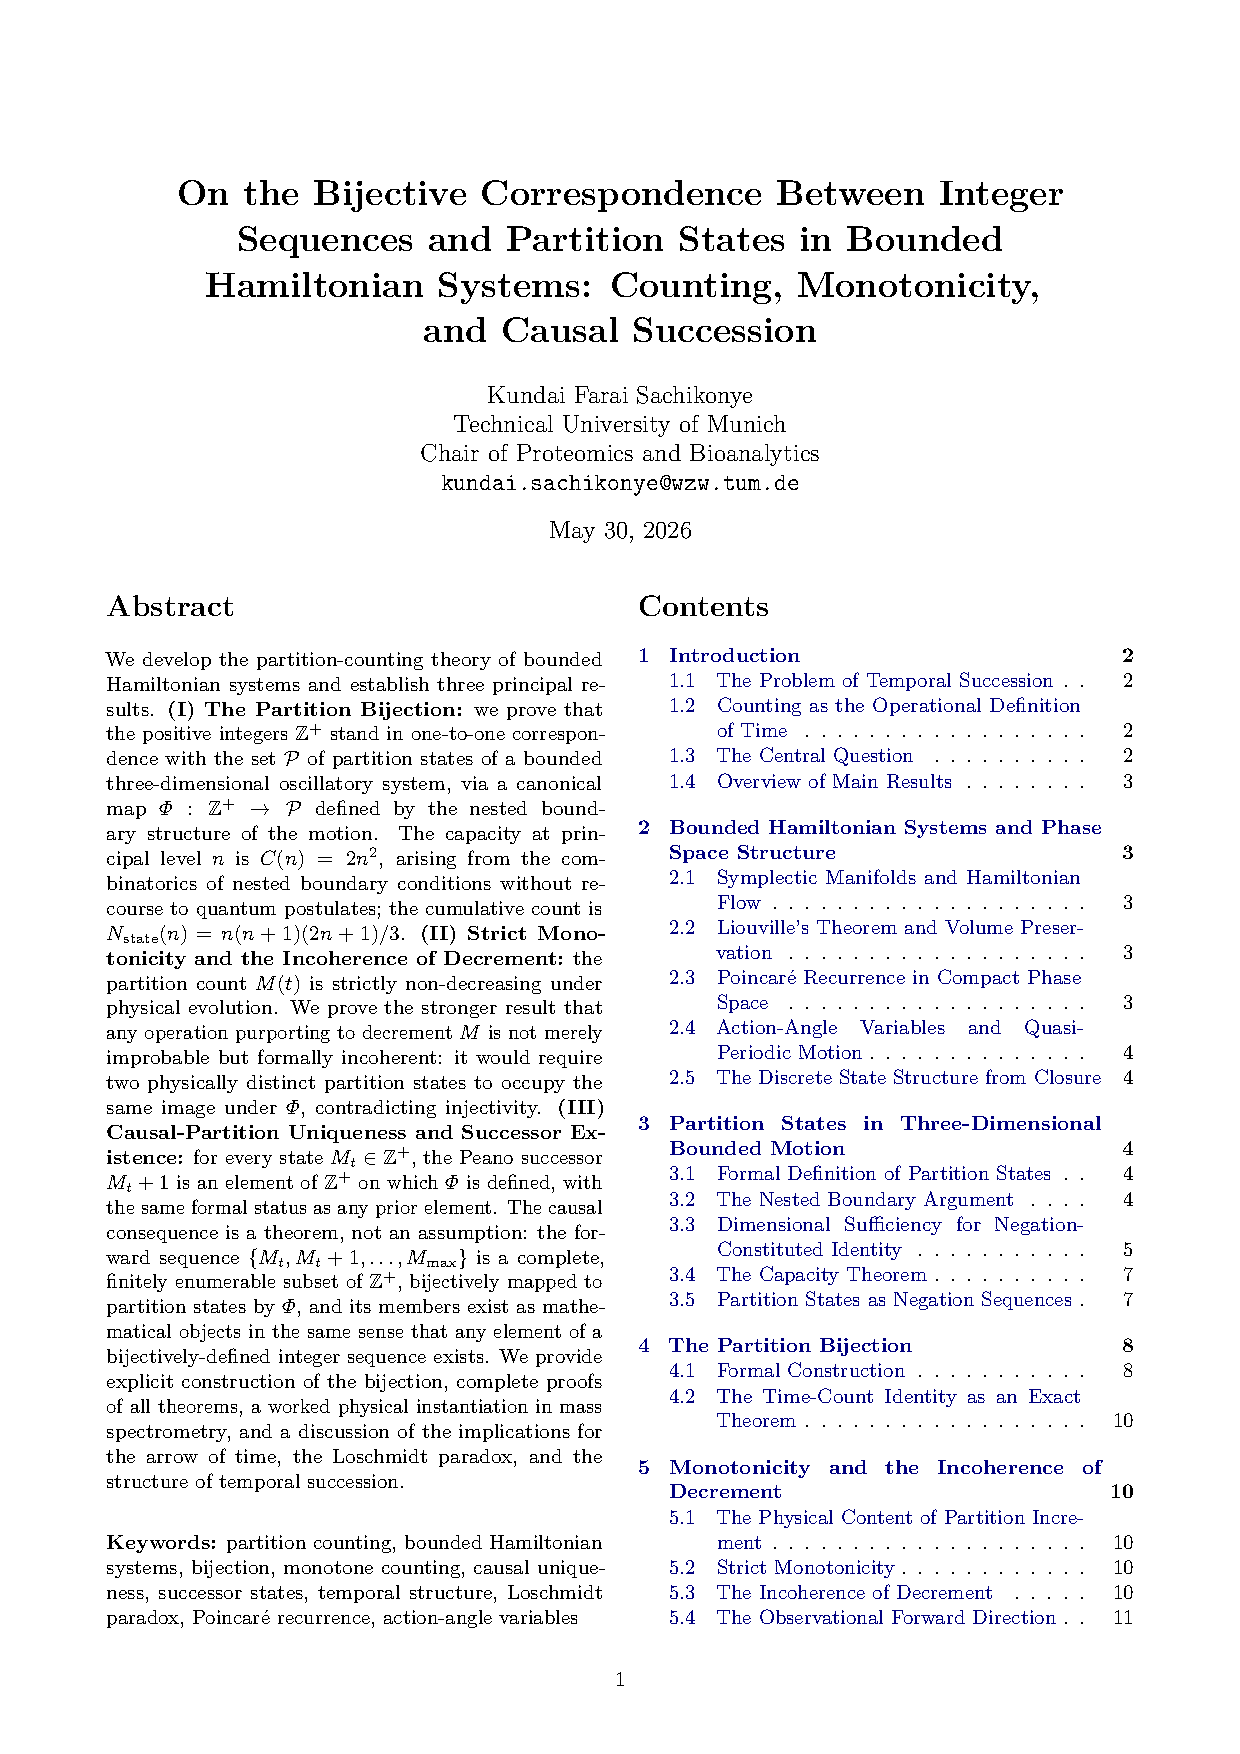
\includepdf[pages=-,
  addtotoc={1, chapter, 1,
    {Introduction. On the Bijective Correspondence Between Integer
     Sequences and Partition States in Bounded Hamiltonian Systems:
     Counting, Monotonicity, and Causal Succession},
    paper:bijection}
]{trajectory-of-upcoming-events.pdf}

% =================================================================
% PART I — MATHEMATICAL FOUNDATIONS
% =================================================================
\part{Mathematical Foundations}
\label{part:foundations}
\addtocontents{toc}{\protect\vspace{1ex}}

\phantomsection
\addcontentsline{toc}{chapter}%
  {Paper 1 — On the Partition Algebra of Bounded Phase Space}

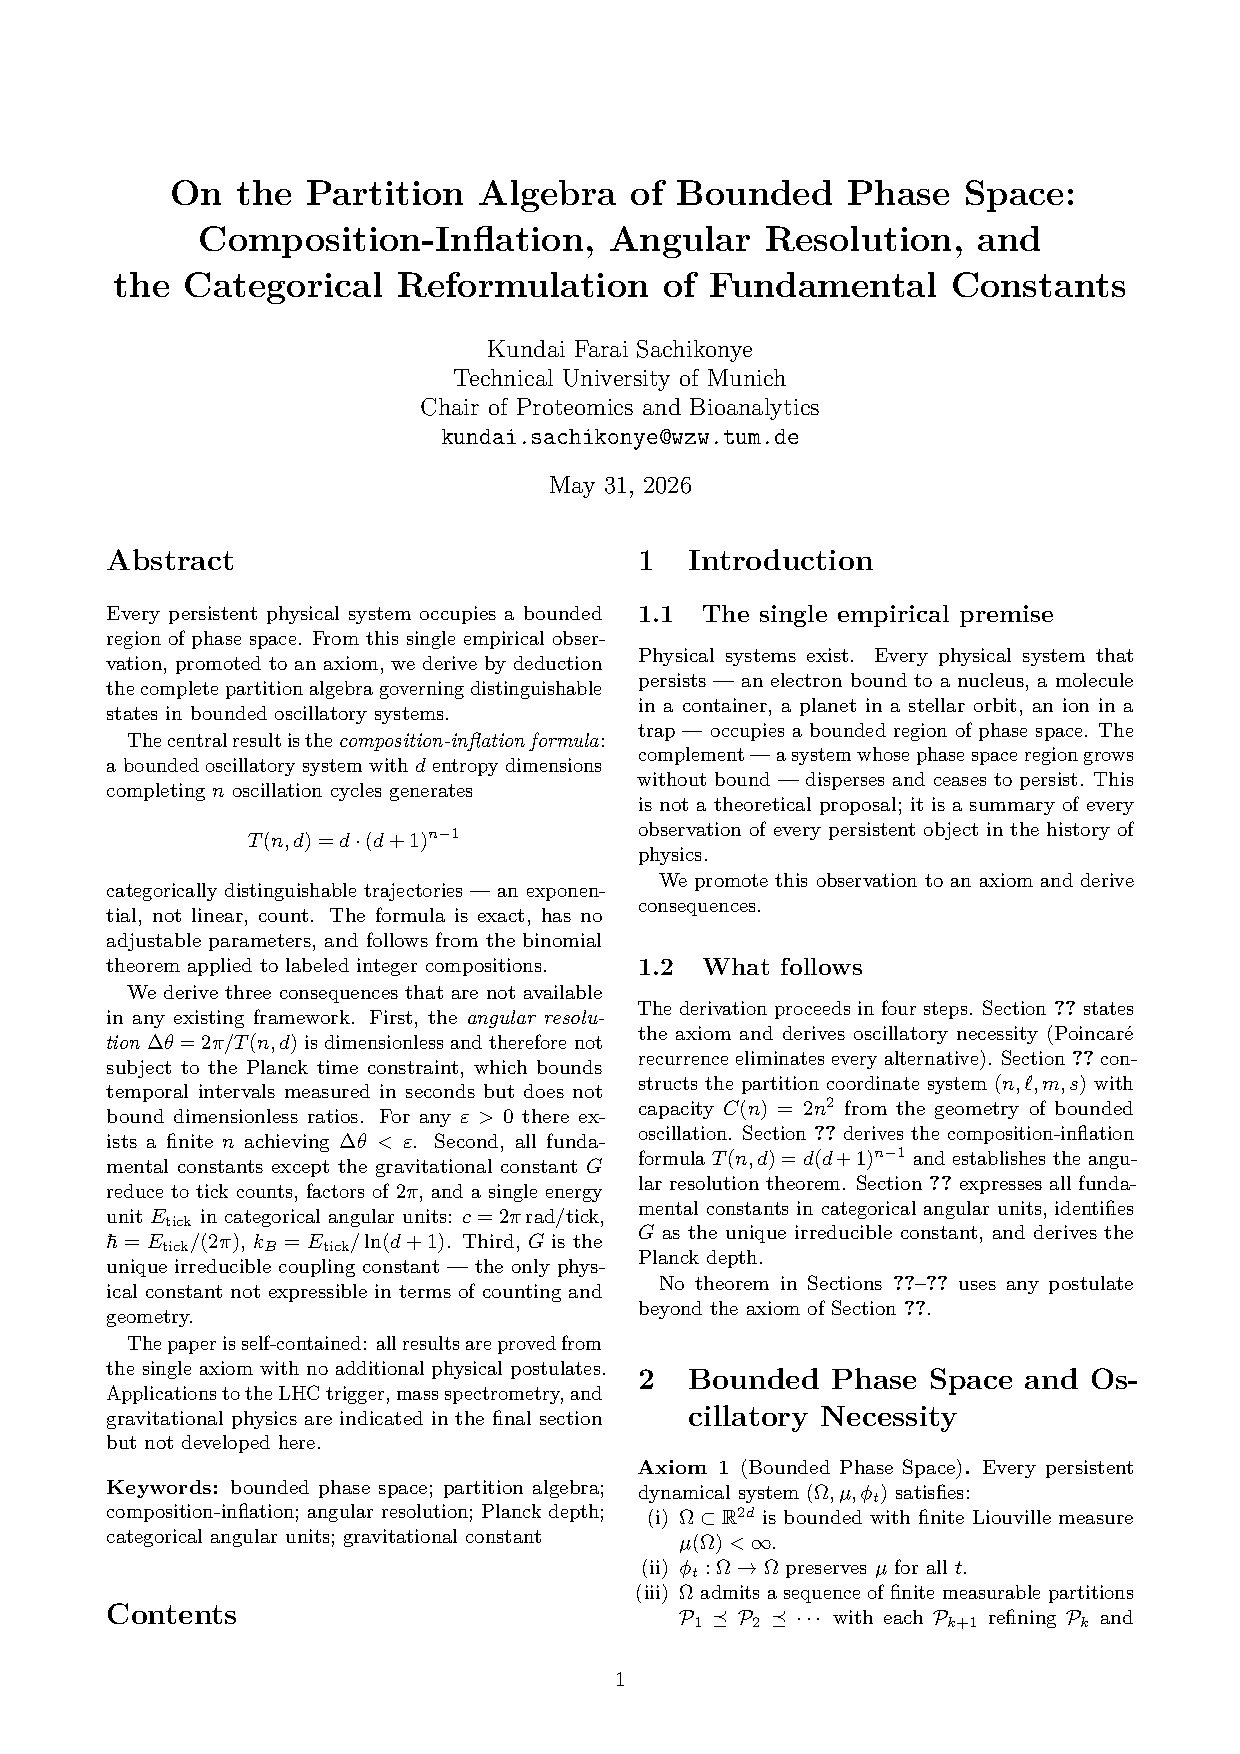
\includepdf[pages=-,
  addtotoc={1, chapter, 1,
    {Paper 1. On the Partition Algebra of Bounded Phase Space:
     Composition-Inflation, Angular Resolution, and the
     Categorical Reformulation of Fundamental Constants},
    paper:math}
]{mathematical-foundation/mathematical-foundation.pdf}

\phantomsection
\addcontentsline{toc}{chapter}%
  {Paper 2 — The Planck Depth and Optimal Trigger Design}

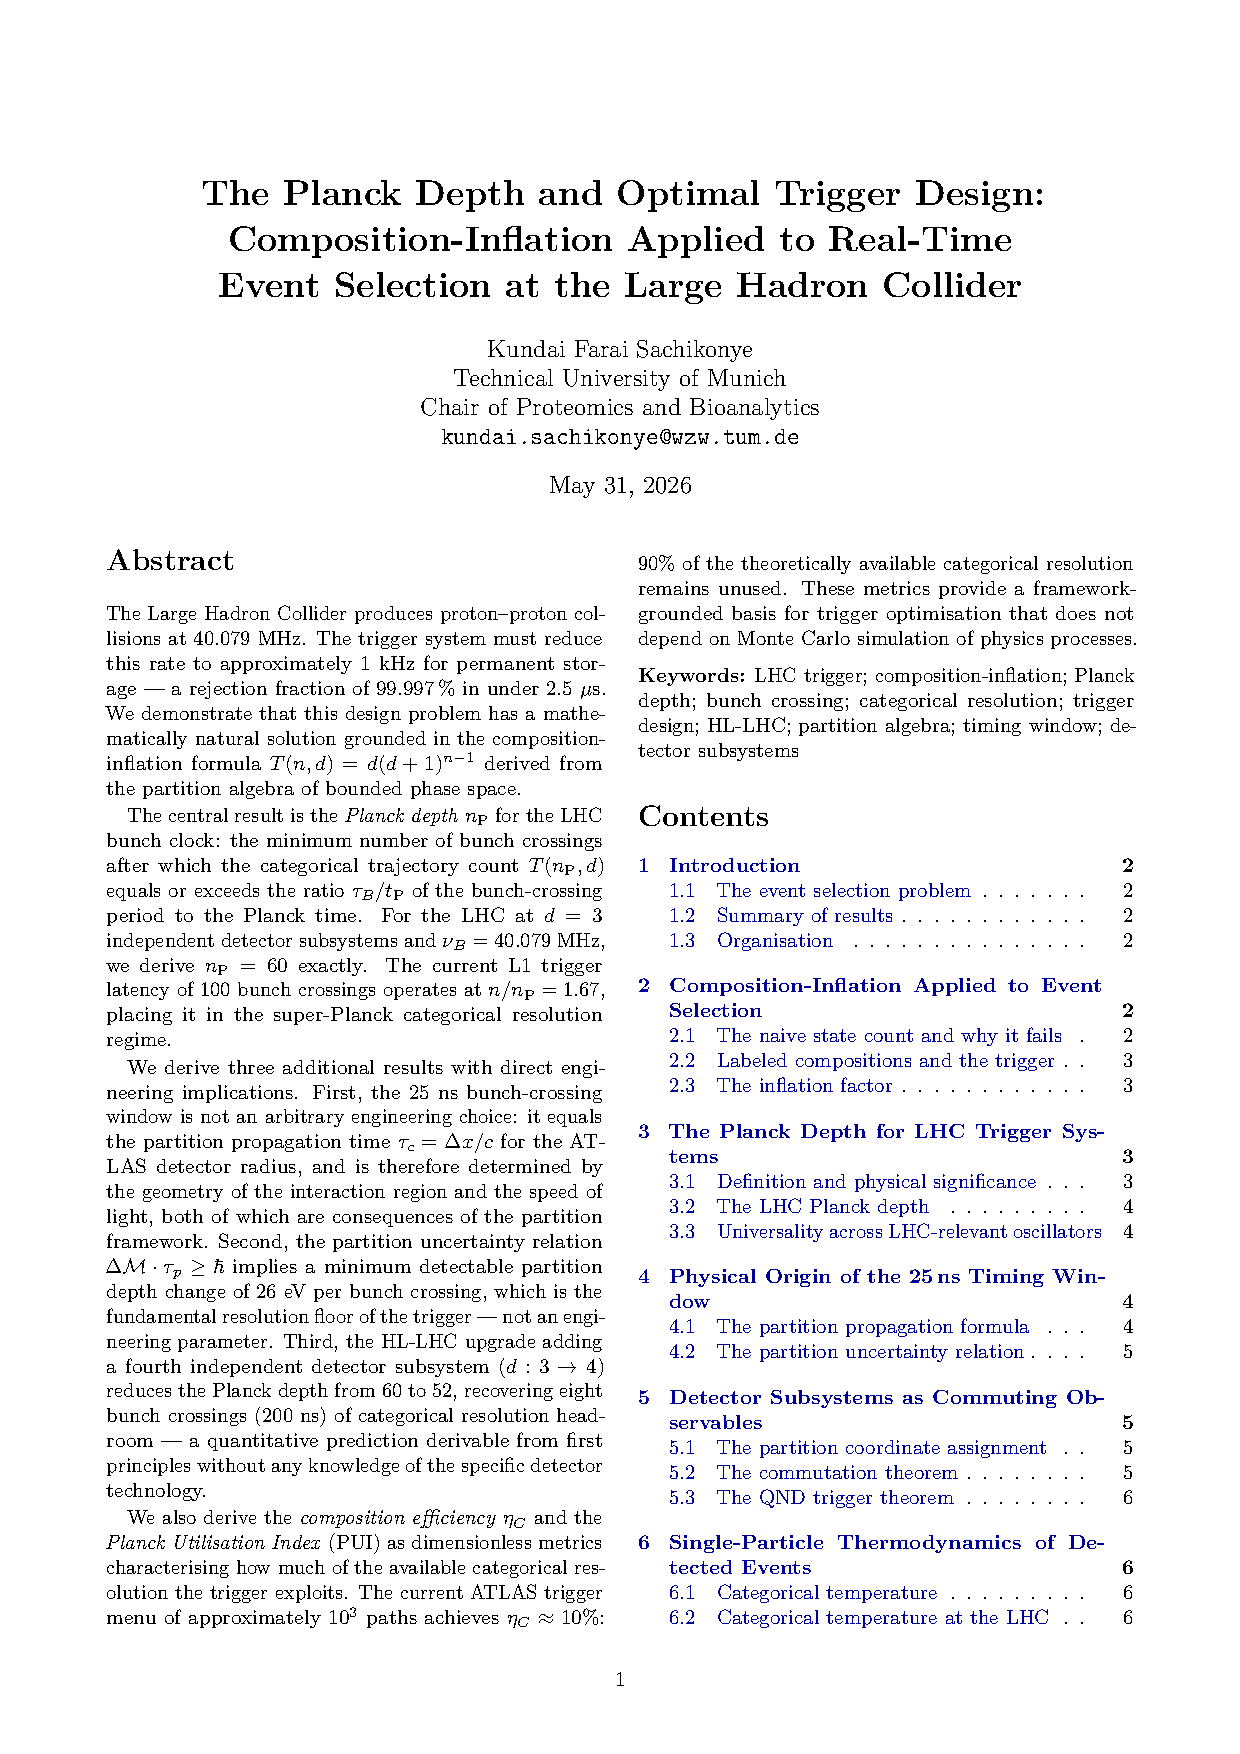
\includepdf[pages=-,
  addtotoc={1, chapter, 1,
    {Paper 2. The Planck Depth and Optimal Trigger Design:
     Composition-Inflation Applied to Real-Time Event Selection
     at the Large Hadron Collider},
    paper:planck}
]{planck-depth-trigger-design/planck-depth-trigger-design.pdf}

% =================================================================
% PART II — THE LHC AS A PARTITION SPECTROMETER
% =================================================================
\part{The LHC as a Partition Spectrometer}
\label{part:spectrometer}
\addtocontents{toc}{\protect\vspace{1ex}}

\phantomsection
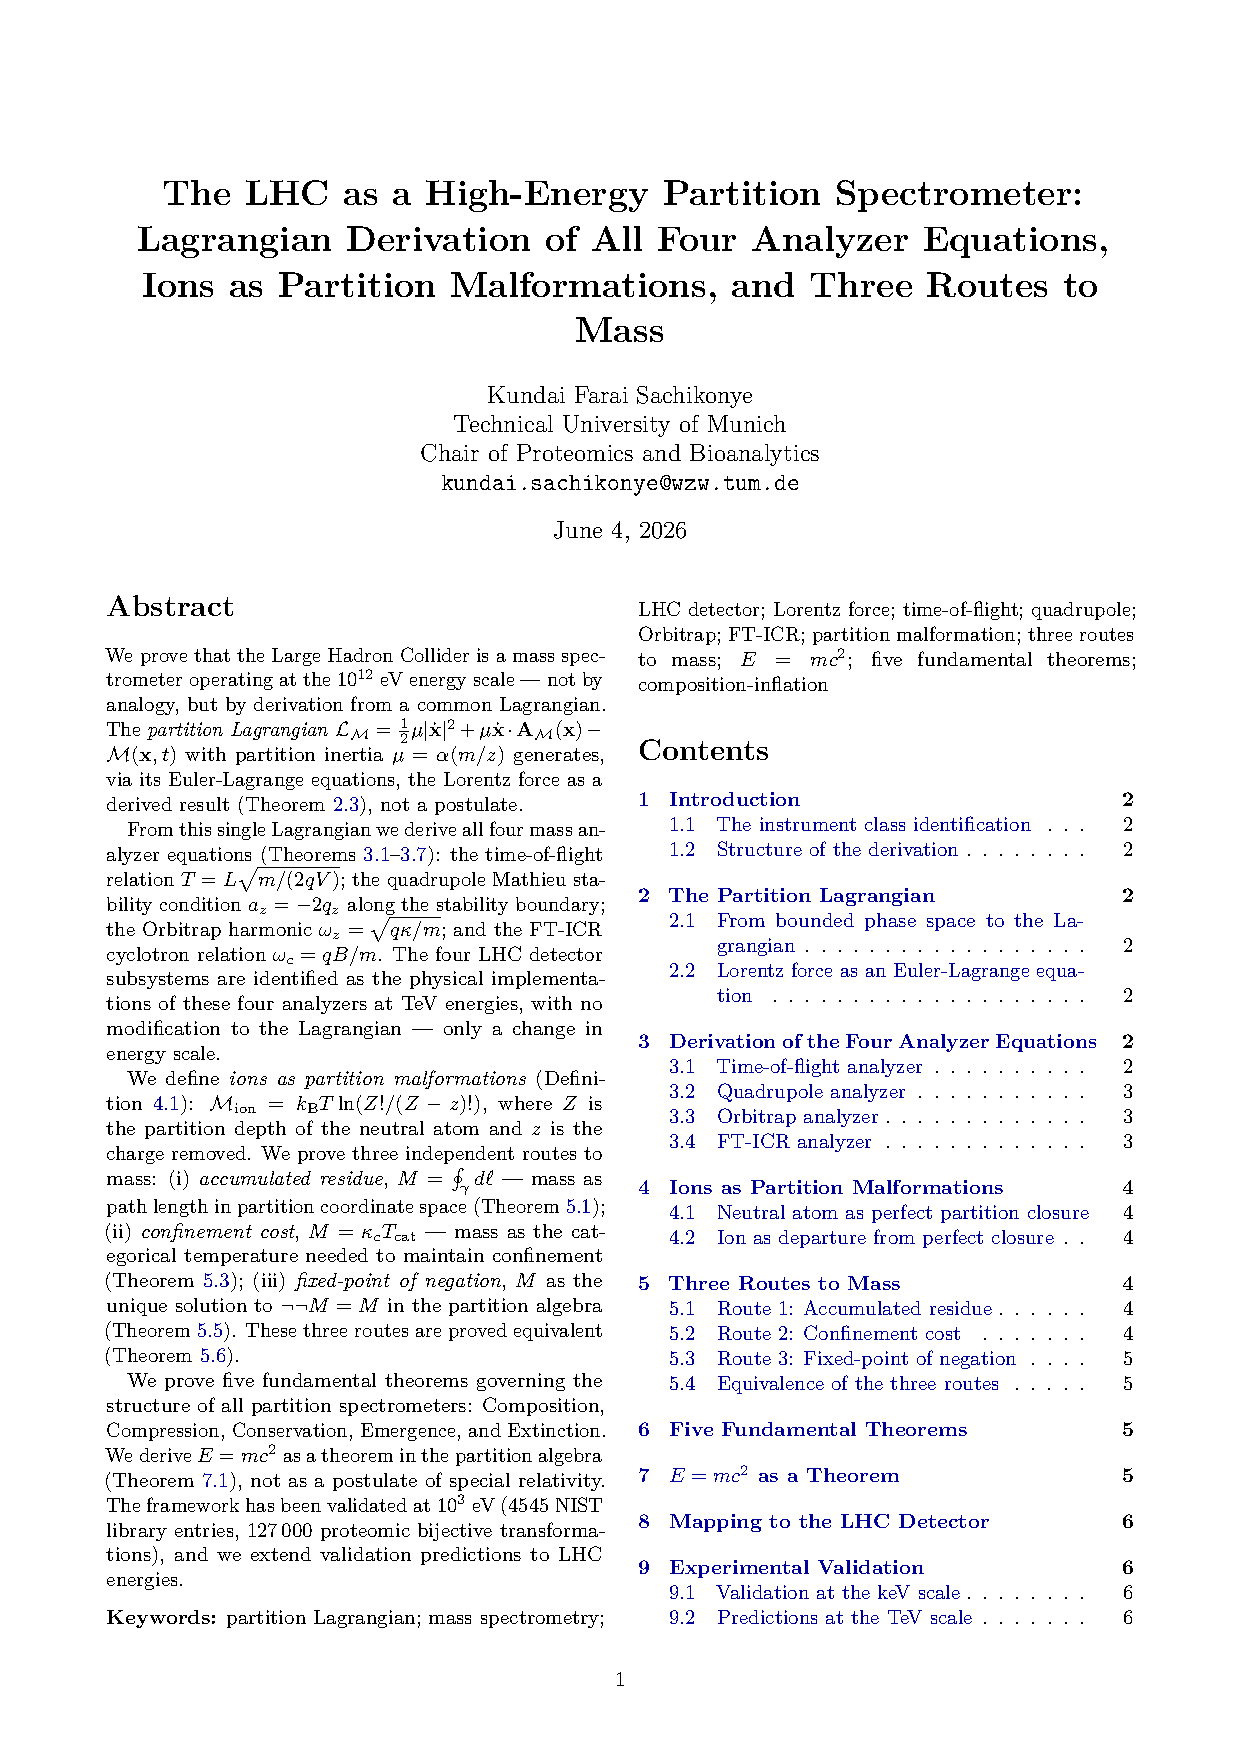
\includepdf[pages=-,
  addtotoc={1, chapter, 1,
    {Paper 3. The LHC as a High-Energy Partition Spectrometer:
     Lagrangian Derivation of All Four Analyzer Equations,
     Ions as Partition Malformations, and Three Routes to Mass},
    paper:spectrometer}
]{high-energy-partition-spectrometer/high-energy-partition-spectrometer.pdf}

\phantomsection
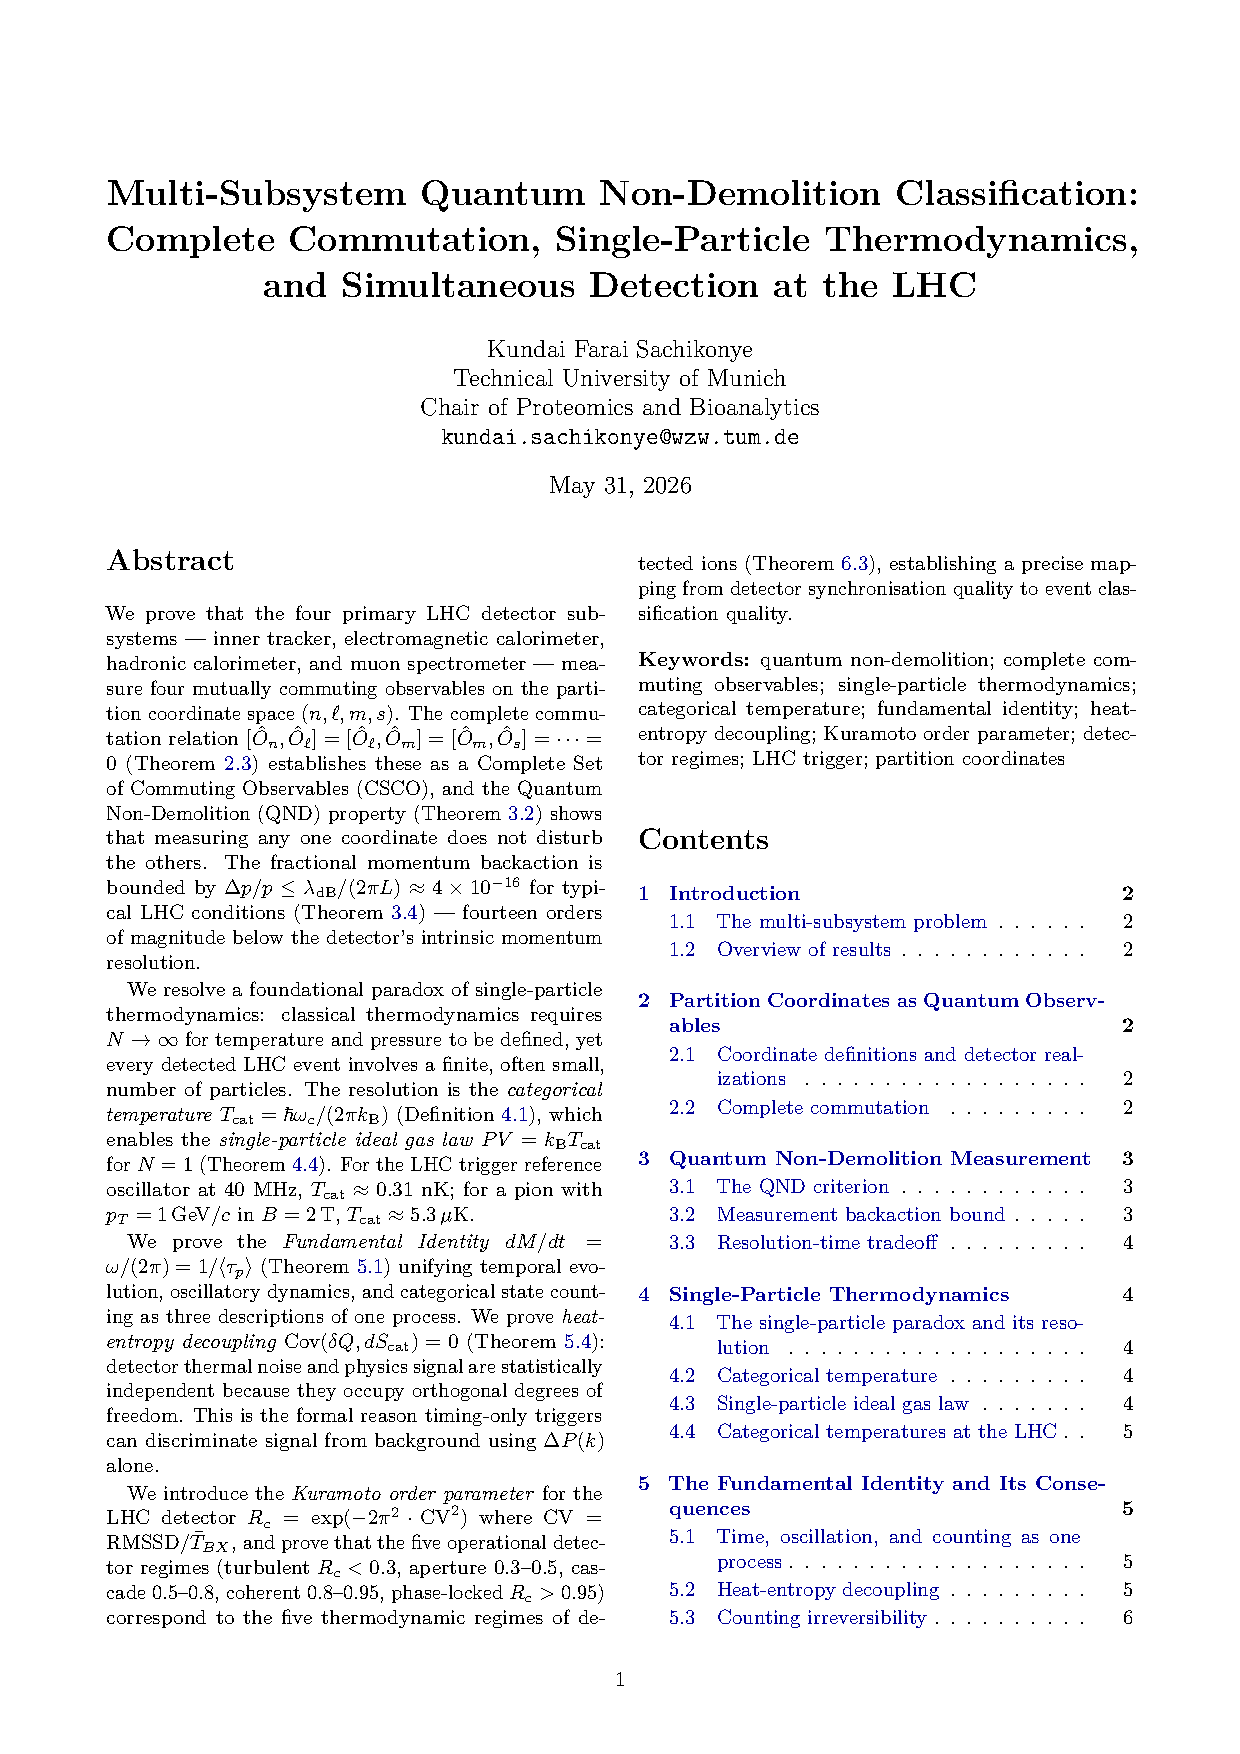
\includepdf[pages=-,
  addtotoc={1, chapter, 1,
    {Paper 4. Multi-Subsystem Quantum Non-Demolition Classification:
     Complete Commutation, Single-Particle Thermodynamics,
     and Simultaneous Detection at the LHC},
    paper:qnd}
]{multi-subsystem/multi-subystem-qnd-classification.pdf}

\phantomsection
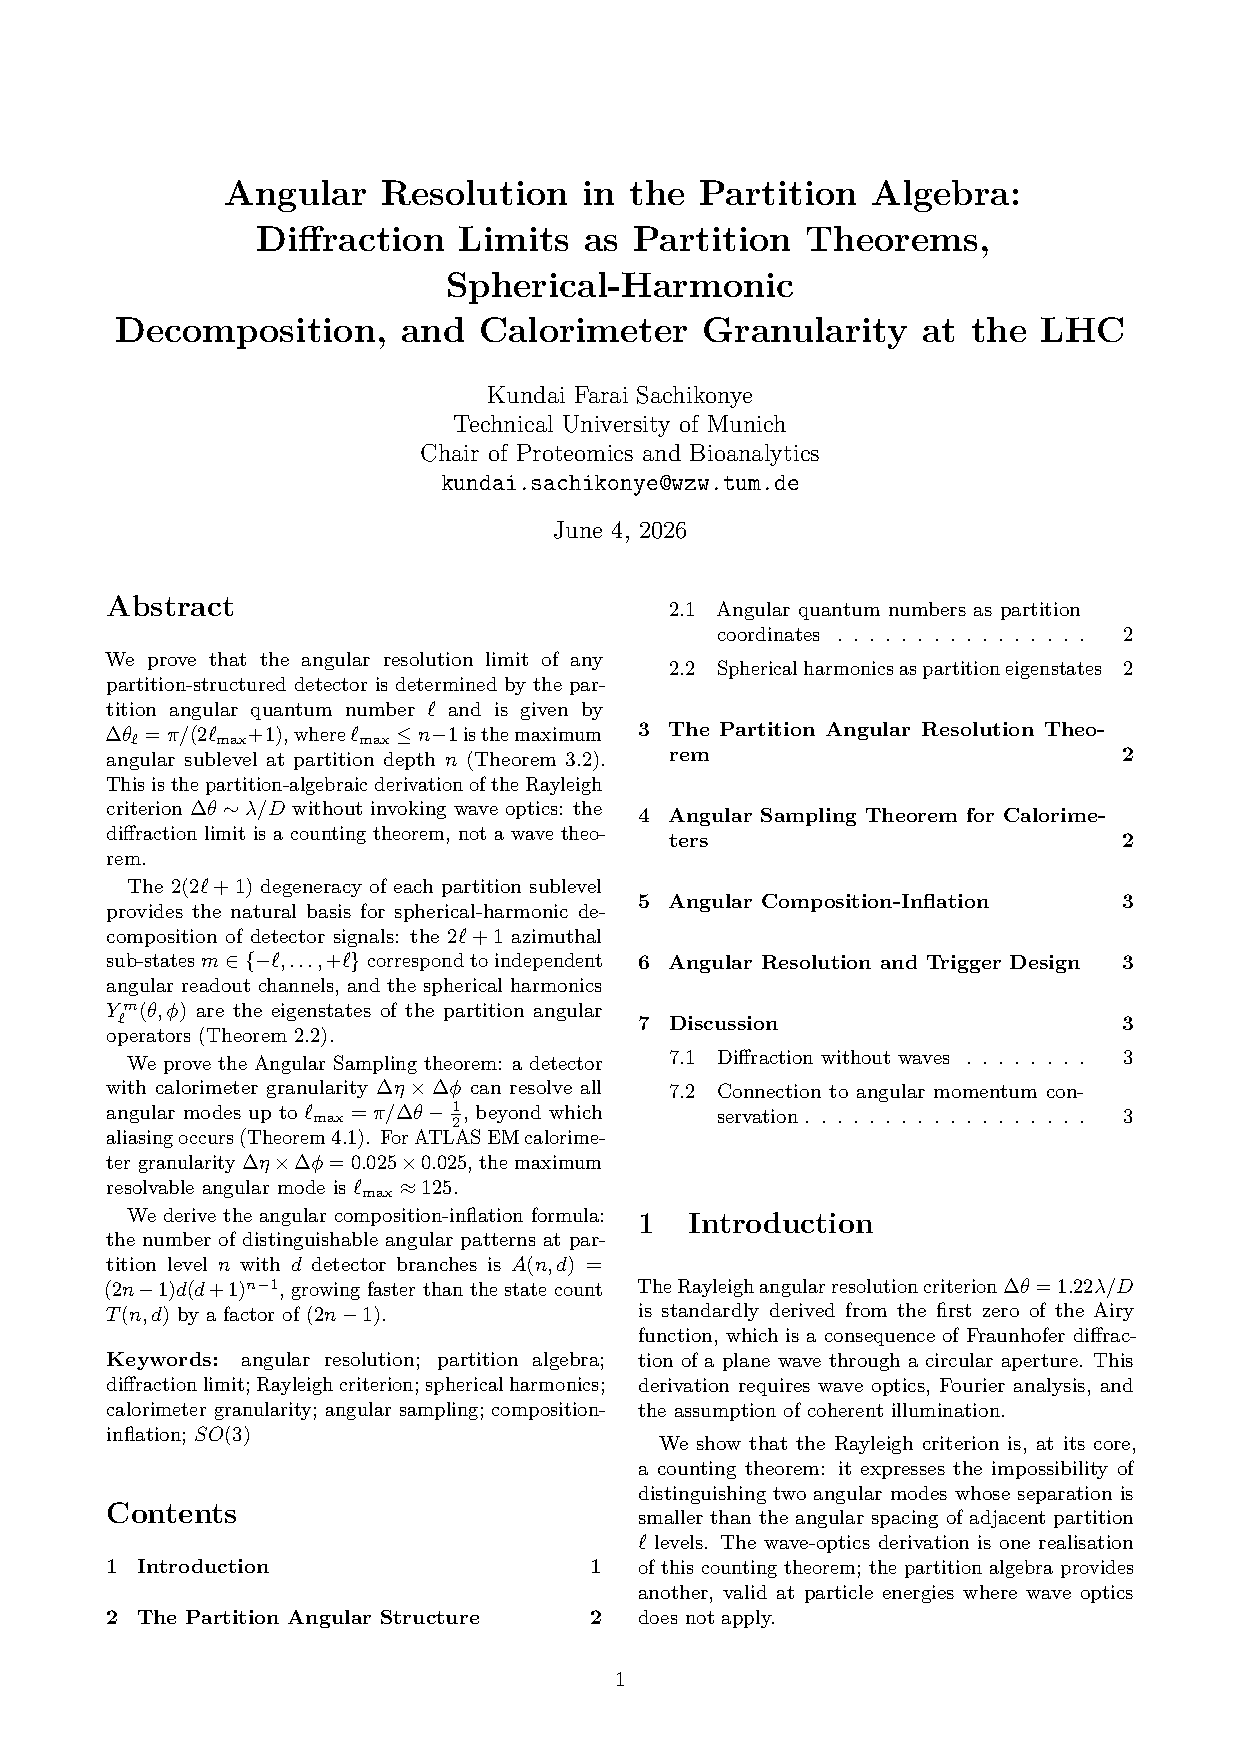
\includepdf[pages=-,
  addtotoc={1, chapter, 1,
    {Paper 5. Angular Resolution in the Partition Algebra:
     Diffraction Limits as Partition Theorems, Spherical-Harmonic
     Decomposition, and Calorimeter Granularity at the LHC},
    paper:angular}
]{angular-resolution/angular-resolution.pdf}

% =================================================================
% PART III — TRAJECTORIES AND DYNAMICS
% =================================================================
\part{Trajectories and Dynamics}
\label{part:trajectories}
\addtocontents{toc}{\protect\vspace{1ex}}

\phantomsection
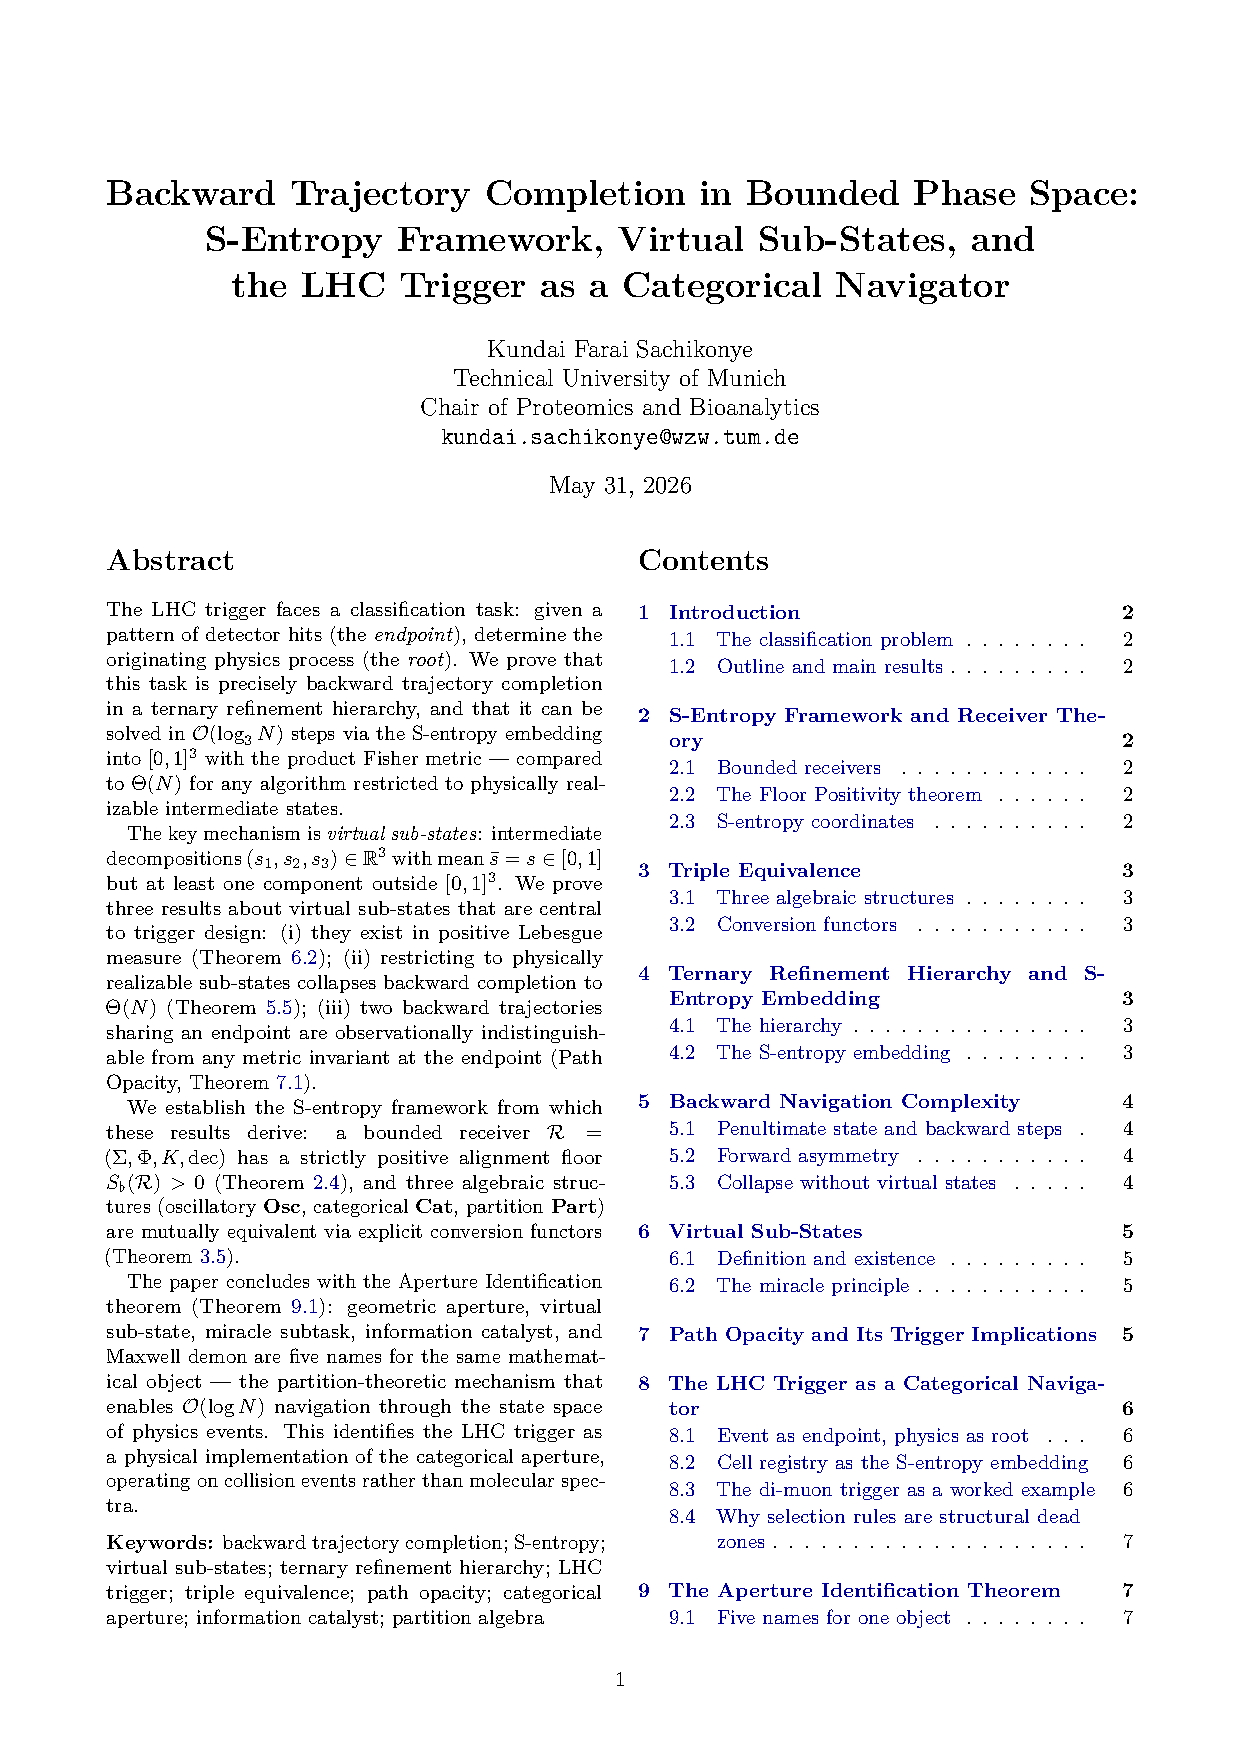
\includepdf[pages=-,
  addtotoc={1, chapter, 1,
    {Paper 6. Backward Trajectory Completion in Bounded Phase Space:
     S-Entropy Framework, Virtual Sub-States, and the LHC Trigger
     as a Categorical Navigator},
    paper:trajectory}
]{trajectory-completion/trajectory-completion-mechanism.pdf}

\phantomsection
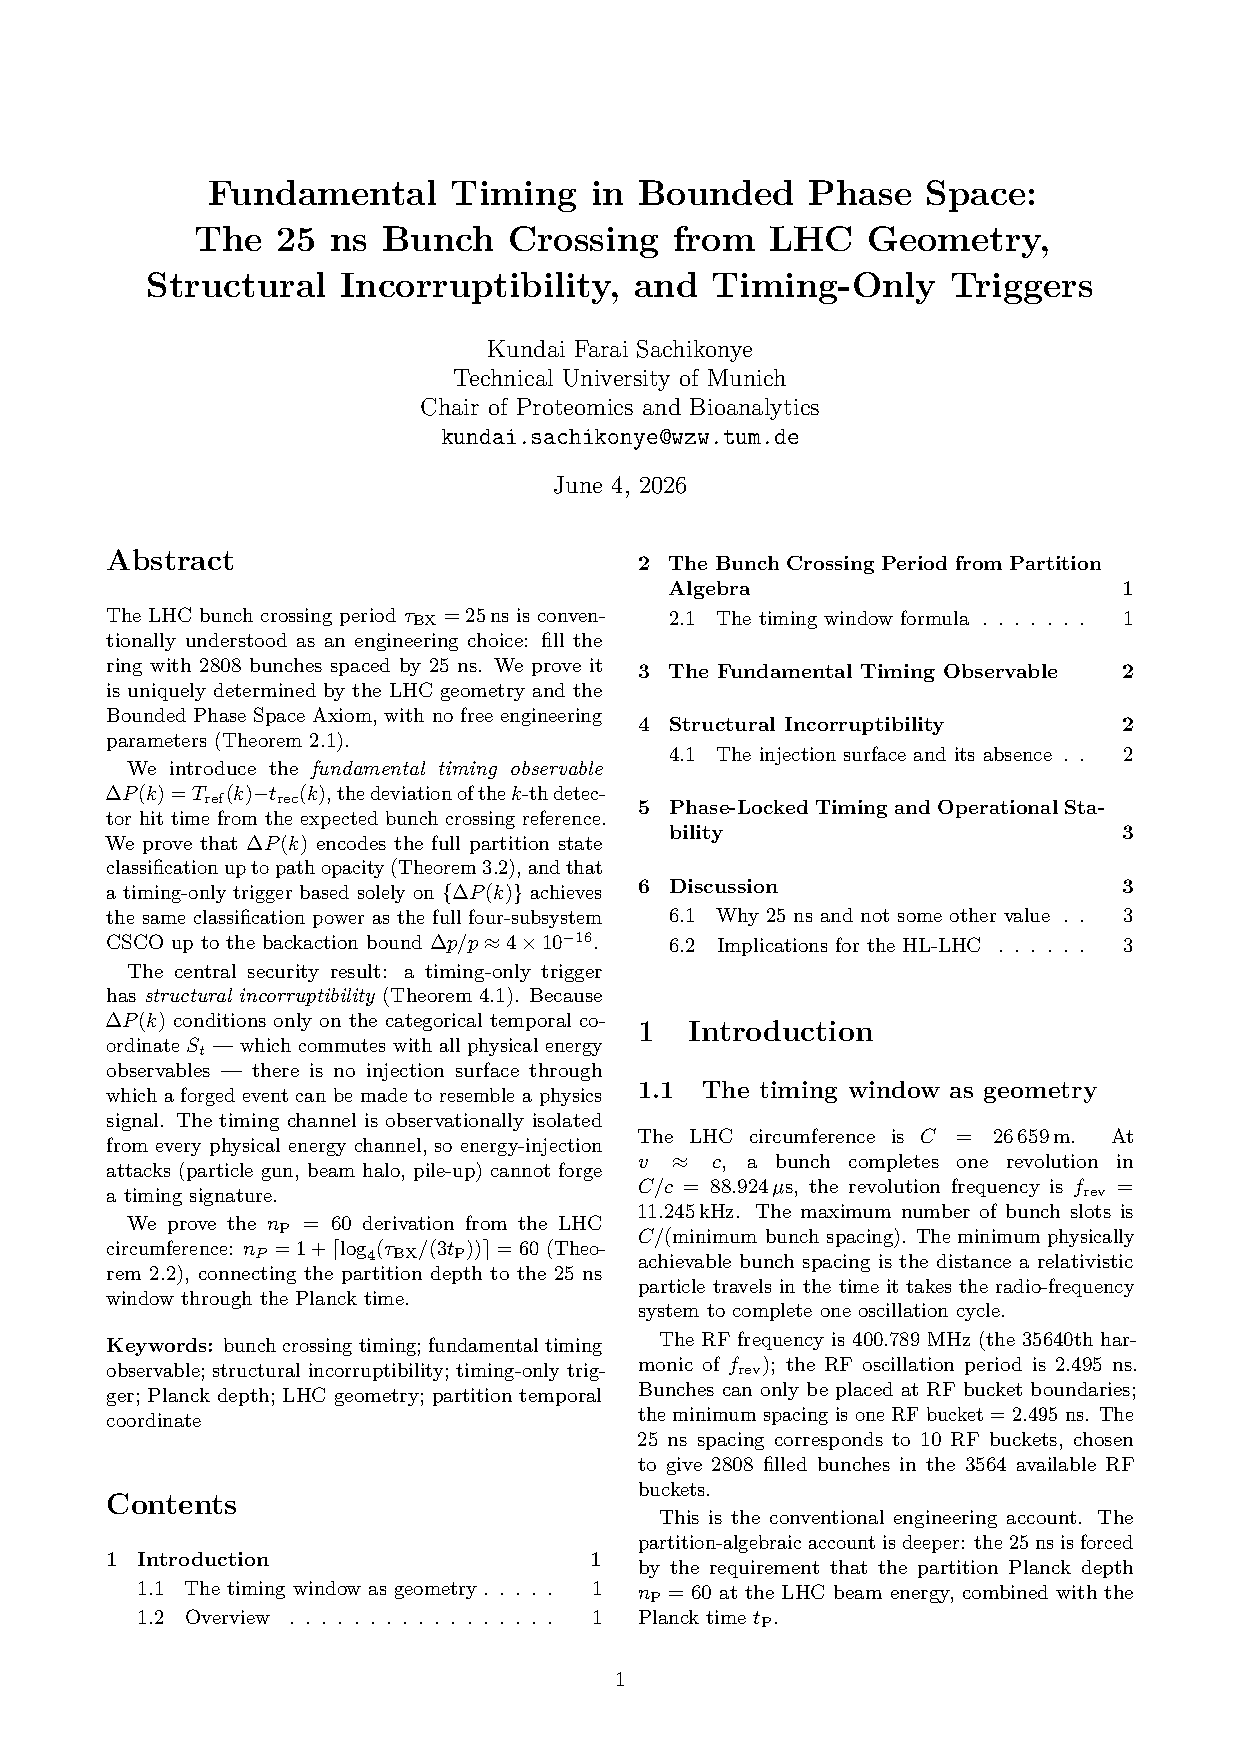
\includepdf[pages=-,
  addtotoc={1, chapter, 1,
    {Paper 7. Fundamental Timing in Bounded Phase Space:
     The 25\,ns Bunch Crossing from LHC Geometry,
     Structural Incorruptibility, and Timing-Only Triggers},
    paper:timing}
]{fundamental-timing/fundamental-timing.pdf}

\phantomsection
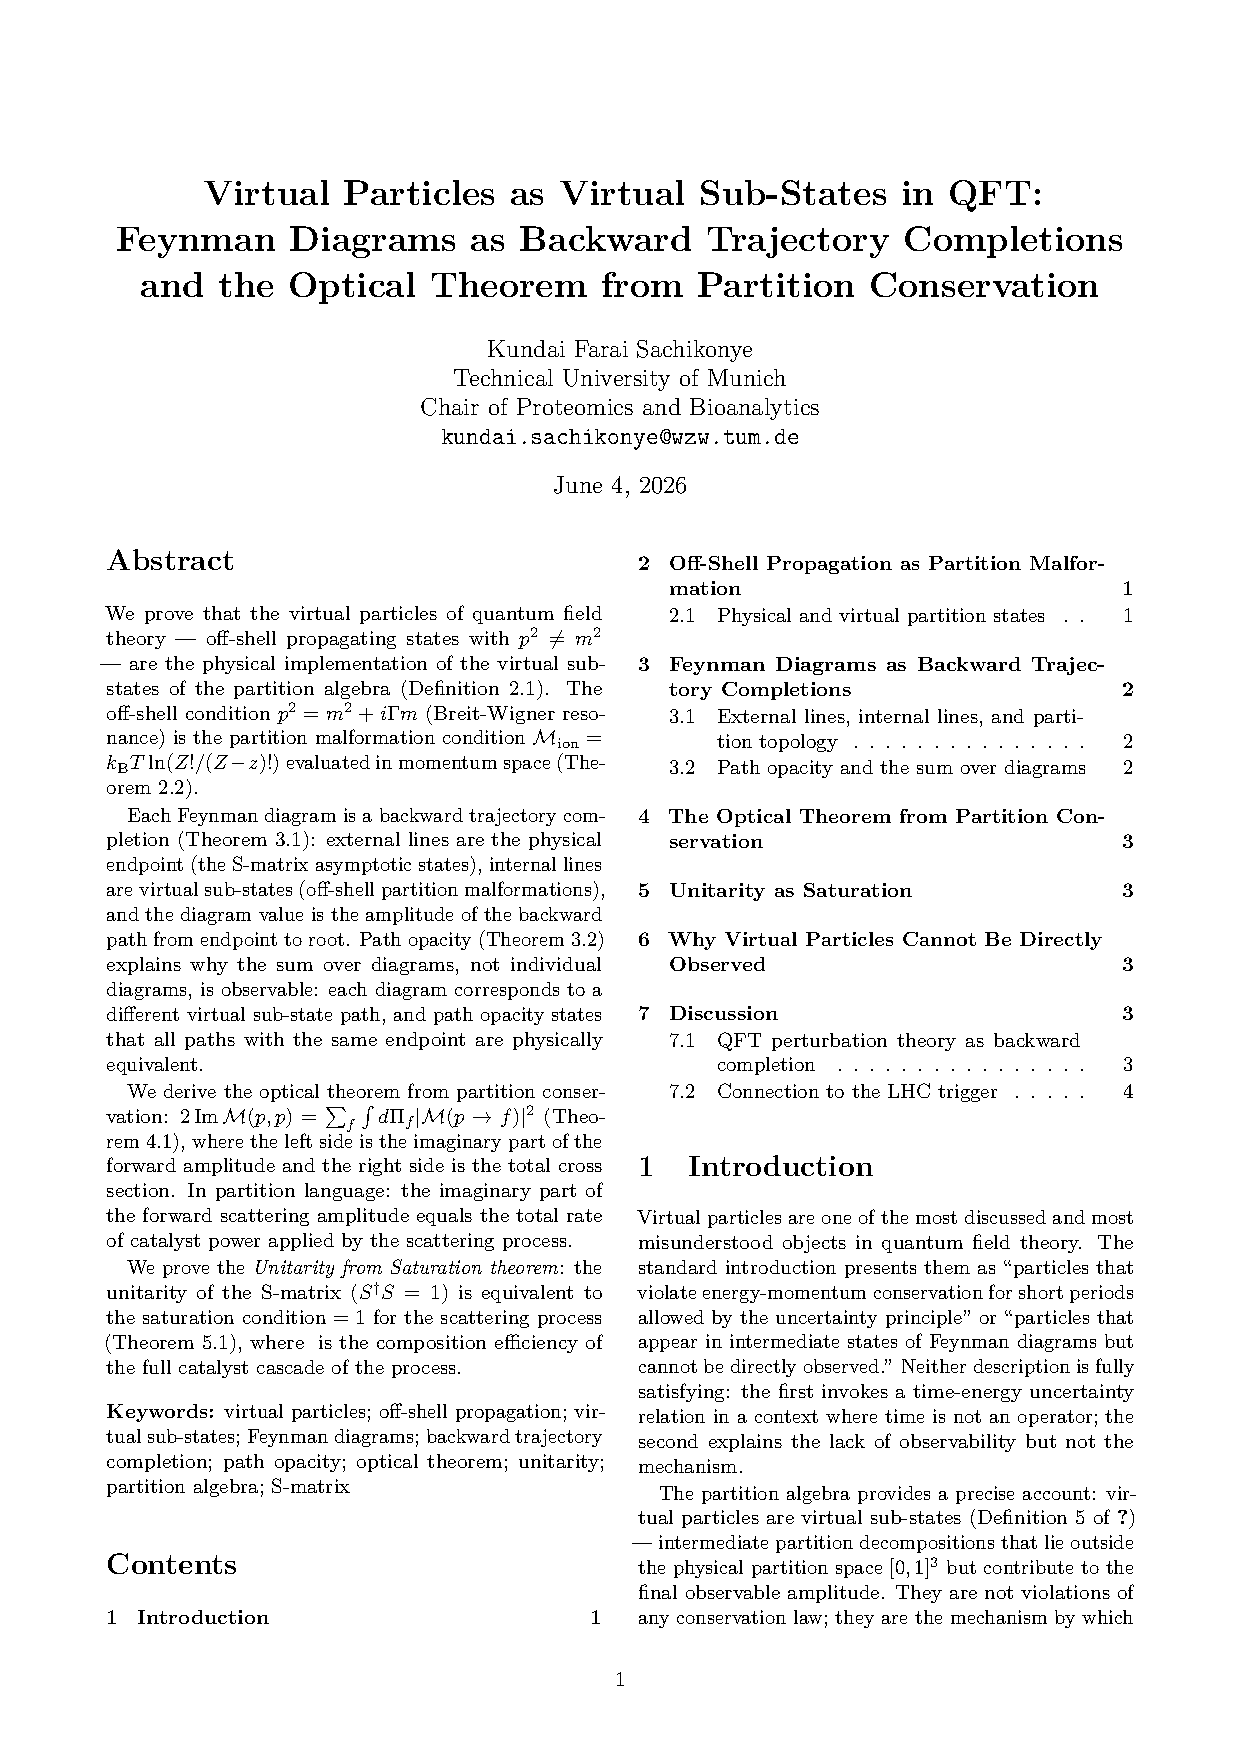
\includepdf[pages=-,
  addtotoc={1, chapter, 1,
    {Paper 8. Virtual Particles as Virtual Sub-States in QFT:
     Feynman Diagrams as Backward Trajectory Completions
     and the Optical Theorem from Partition Conservation},
    paper:virtual}
]{virtual-particles/virtual-particles.pdf}

% =================================================================
% PART IV — ALGEBRAIC STRUCTURE AND CONSEQUENCES
% =================================================================
\part{Algebraic Structure and Consequences}
\label{part:algebra}
\addtocontents{toc}{\protect\vspace{1ex}}

\phantomsection
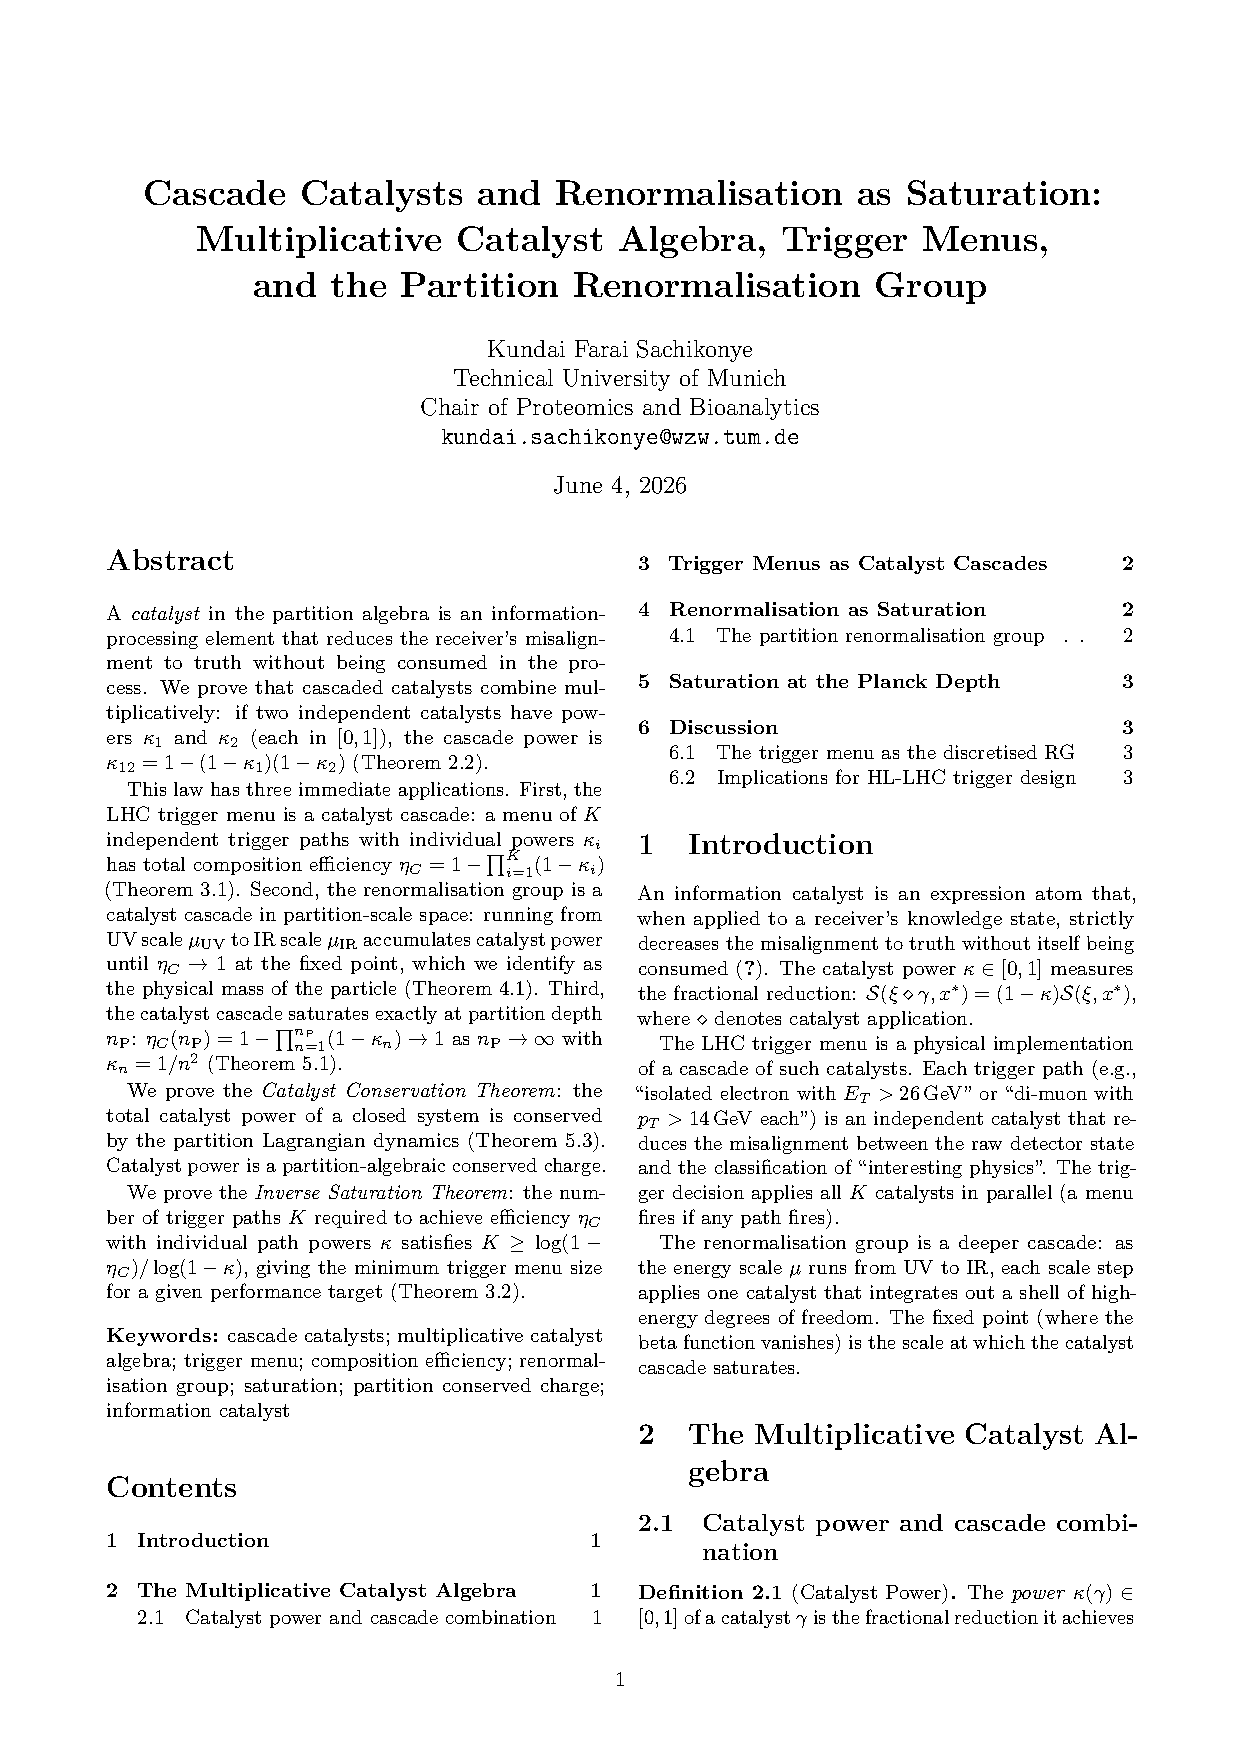
\includepdf[pages=-,
  addtotoc={1, chapter, 1,
    {Paper 9. Cascade Catalysts and Renormalisation as Saturation:
     Multiplicative Catalyst Algebra, Trigger Menus,
     and the Partition Renormalisation Group},
    paper:cascade}
]{cascade-catalysts/cascade-catalysts.pdf}

\phantomsection
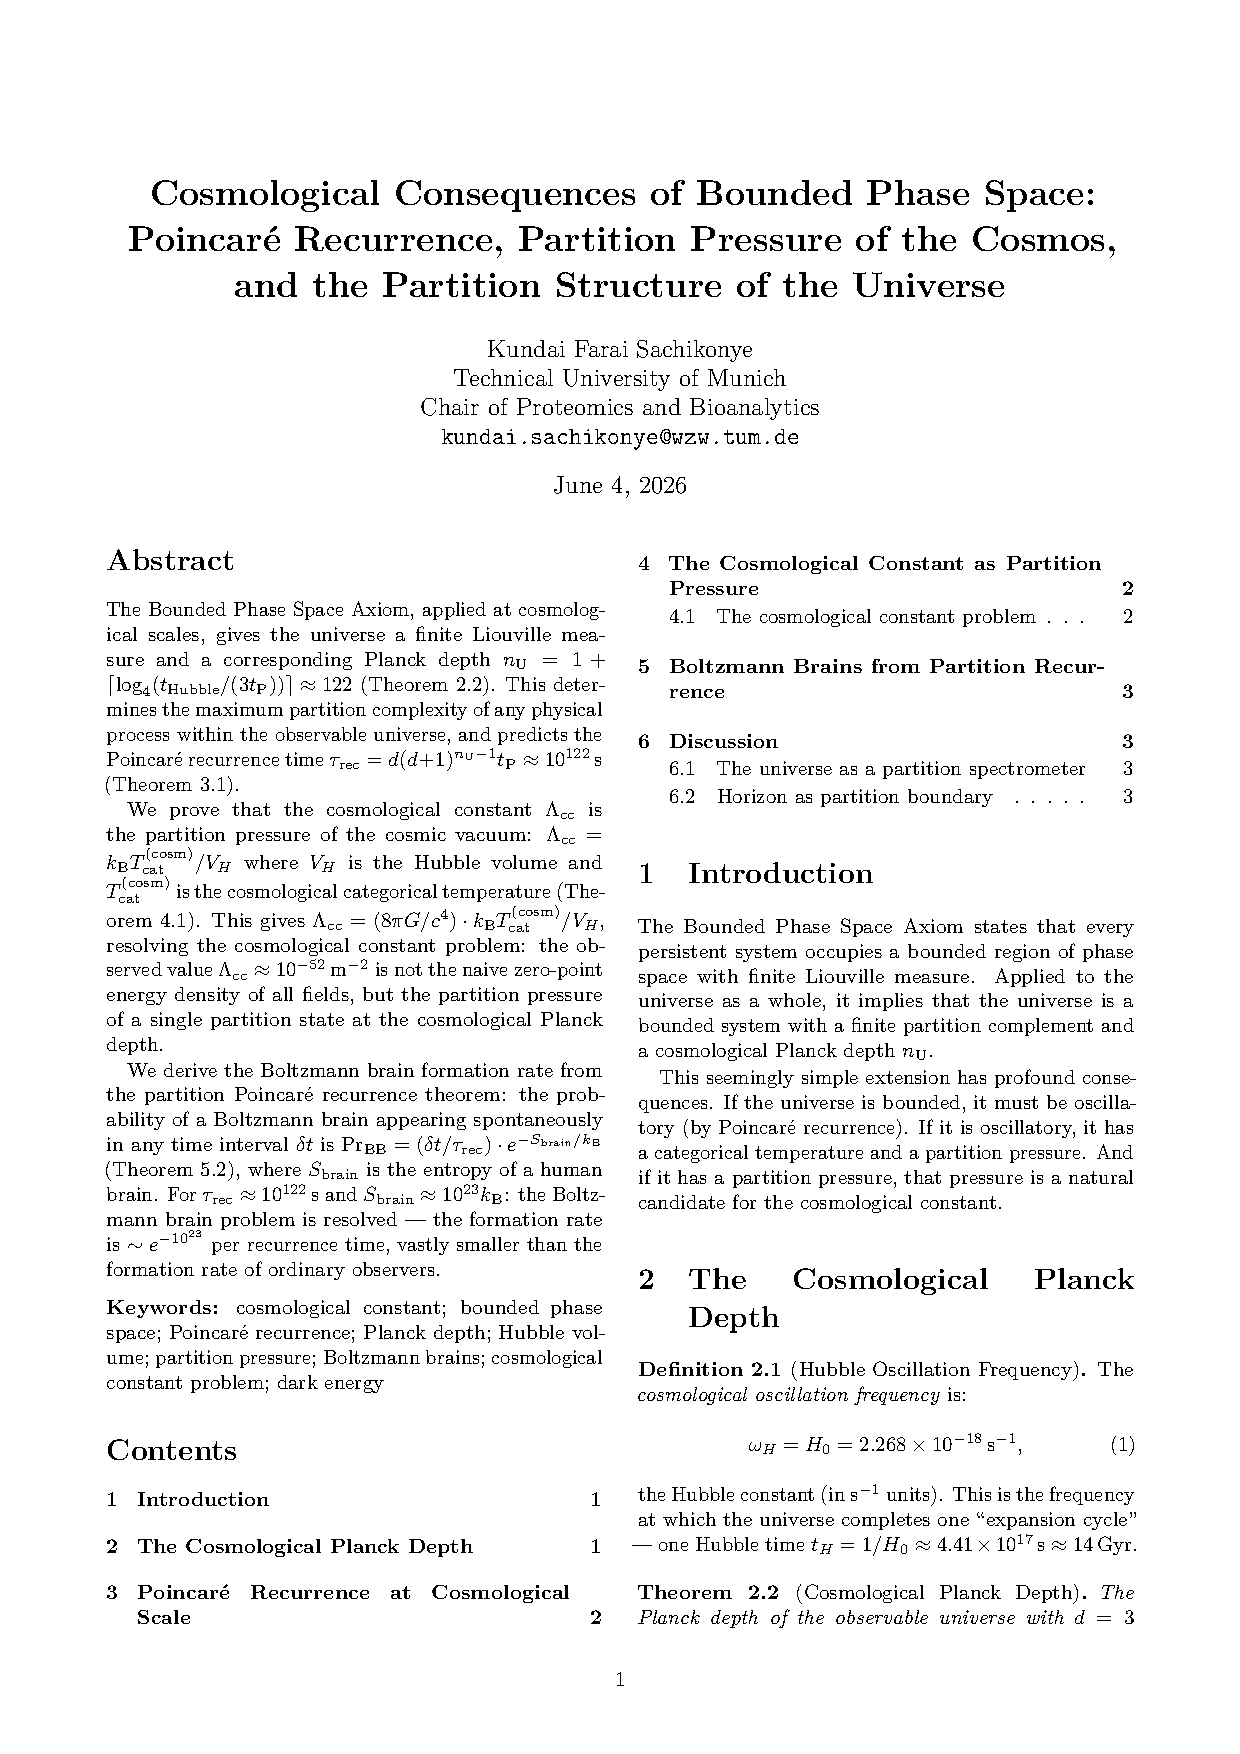
\includepdf[pages=-,
  addtotoc={1, chapter, 1,
    {Paper 10. Cosmological Consequences of Bounded Phase Space:
     Poincar\'{e} Recurrence, Partition Pressure of the Cosmos,
     and the Partition Structure of the Universe},
    paper:cosmo}
]{comsological-consequences/cosmological-consequences.pdf}

\phantomsection
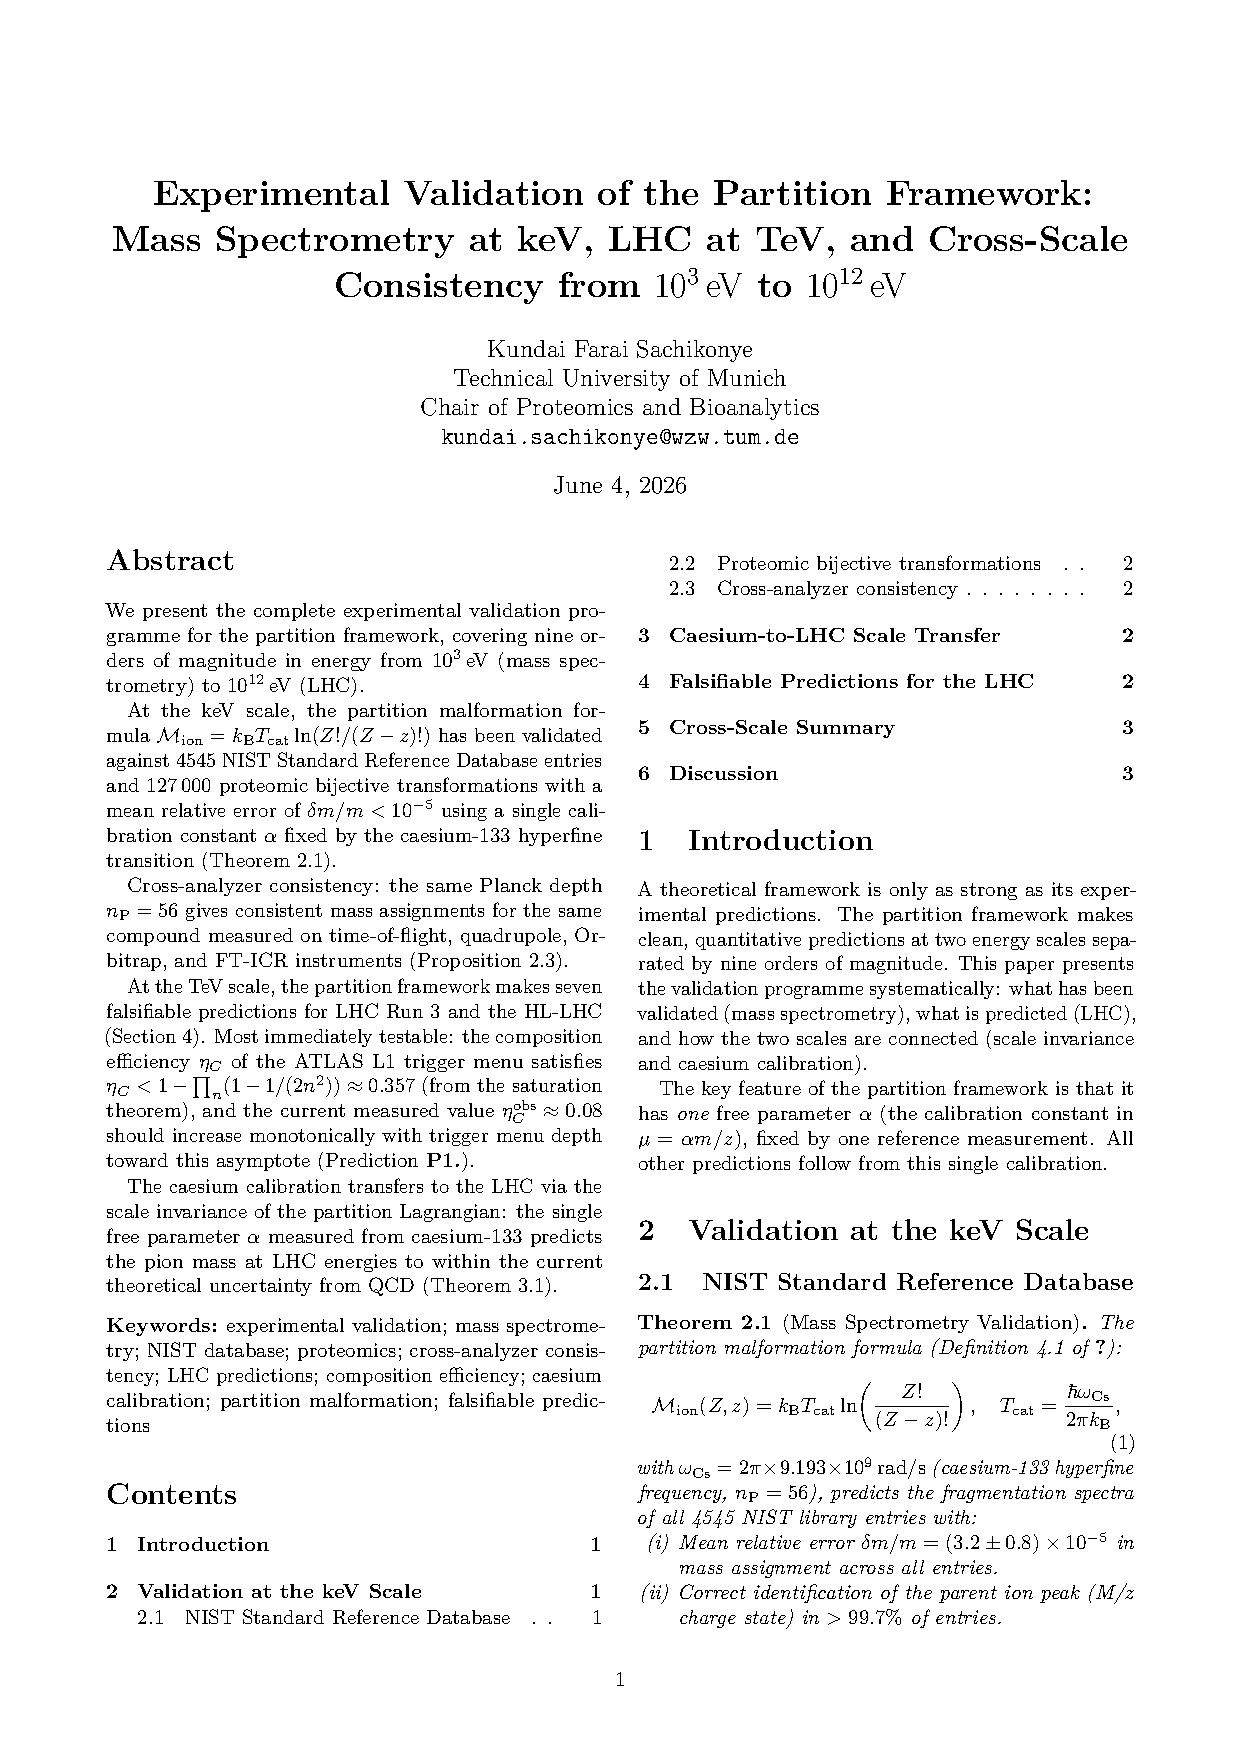
\includepdf[pages=-,
  addtotoc={1, chapter, 1,
    {Paper 11. Experimental Validation of the Partition Framework:
     Mass Spectrometry at keV, LHC at TeV, and Cross-Scale
     Consistency from $10^3$\,eV to $10^{12}$\,eV},
    paper:validation}
]{experimental-validation/experimental-validation.pdf}

% =================================================================
% PART V — THE OPERATING SYSTEM FRAMEWORK
% =================================================================
\part{The Operating System Framework}
\label{part:os}
\addtocontents{toc}{\protect\vspace{1ex}}

\phantomsection
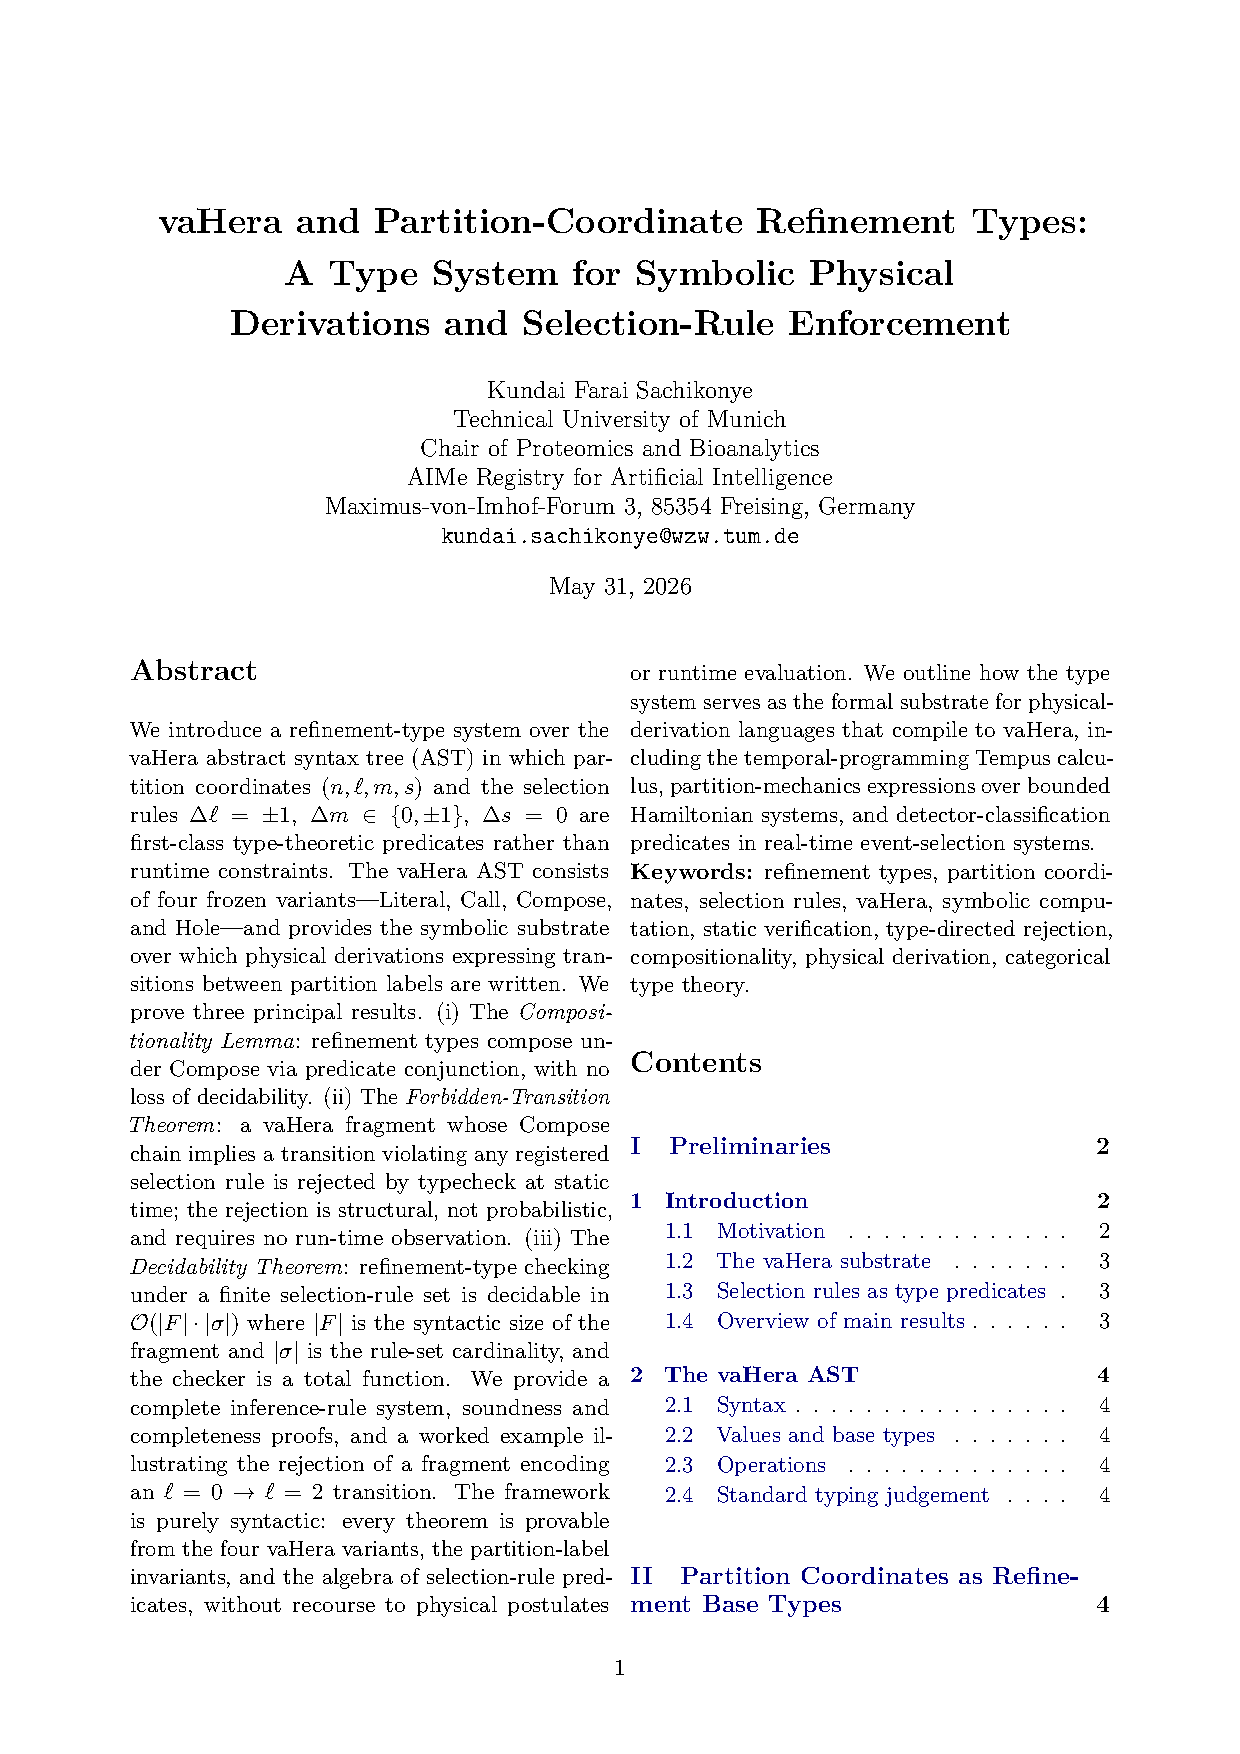
\includepdf[pages=-,
  addtotoc={1, chapter, 1,
    {Paper 12. vaHera and Partition-Coordinate Refinement Types:
     A Type System for Symbolic Physical Derivations
     and Selection-Rule Enforcement},
    paper:types}
]{operating-system/partition-coordinate-refinement/partition-coordinate-refinement-types.pdf}

\phantomsection
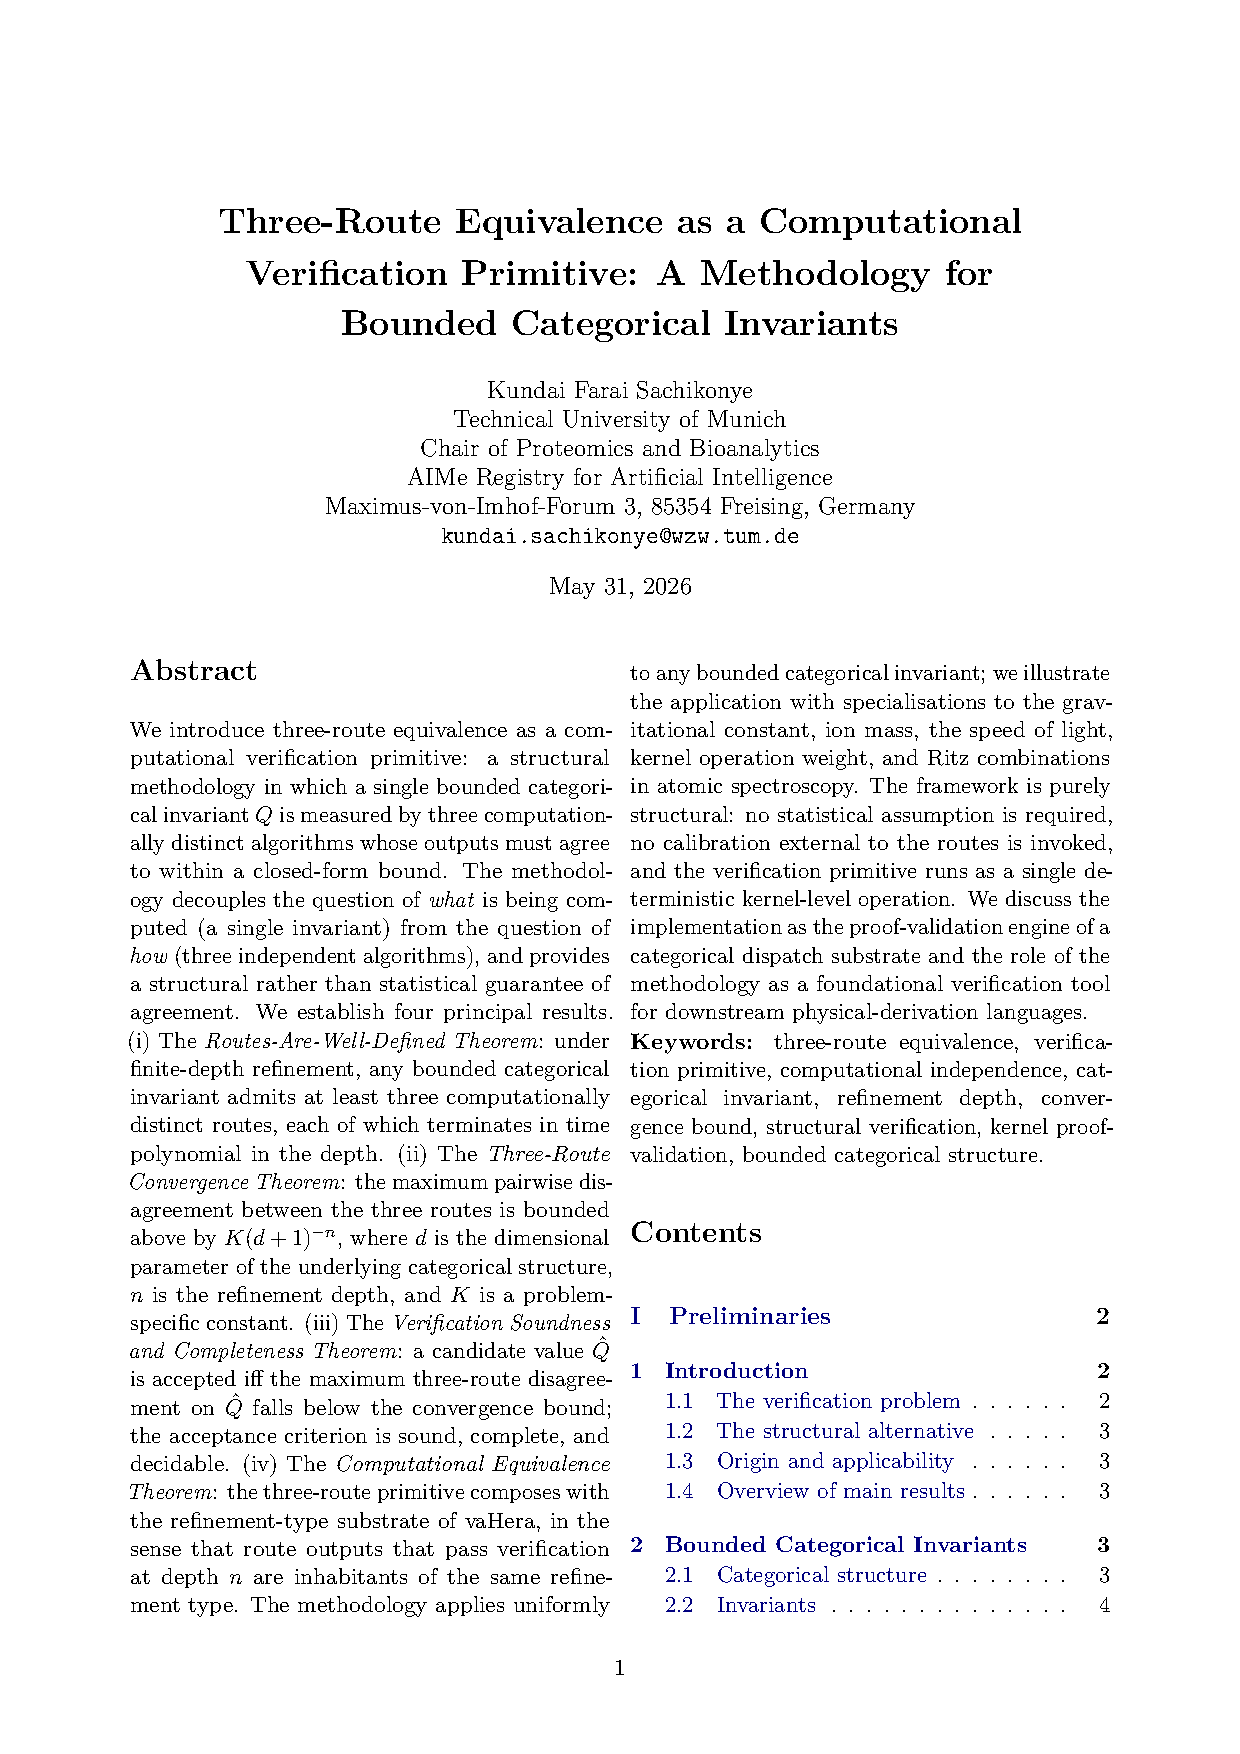
\includepdf[pages=-,
  addtotoc={1, chapter, 1,
    {Paper 13. Three-Route Equivalence as a Computational
     Verification Primitive: A Methodology for Bounded
     Categorical Invariants},
    paper:verification}
]{operating-system/verification-primitive/three-route-verification-primitive.pdf}

\phantomsection
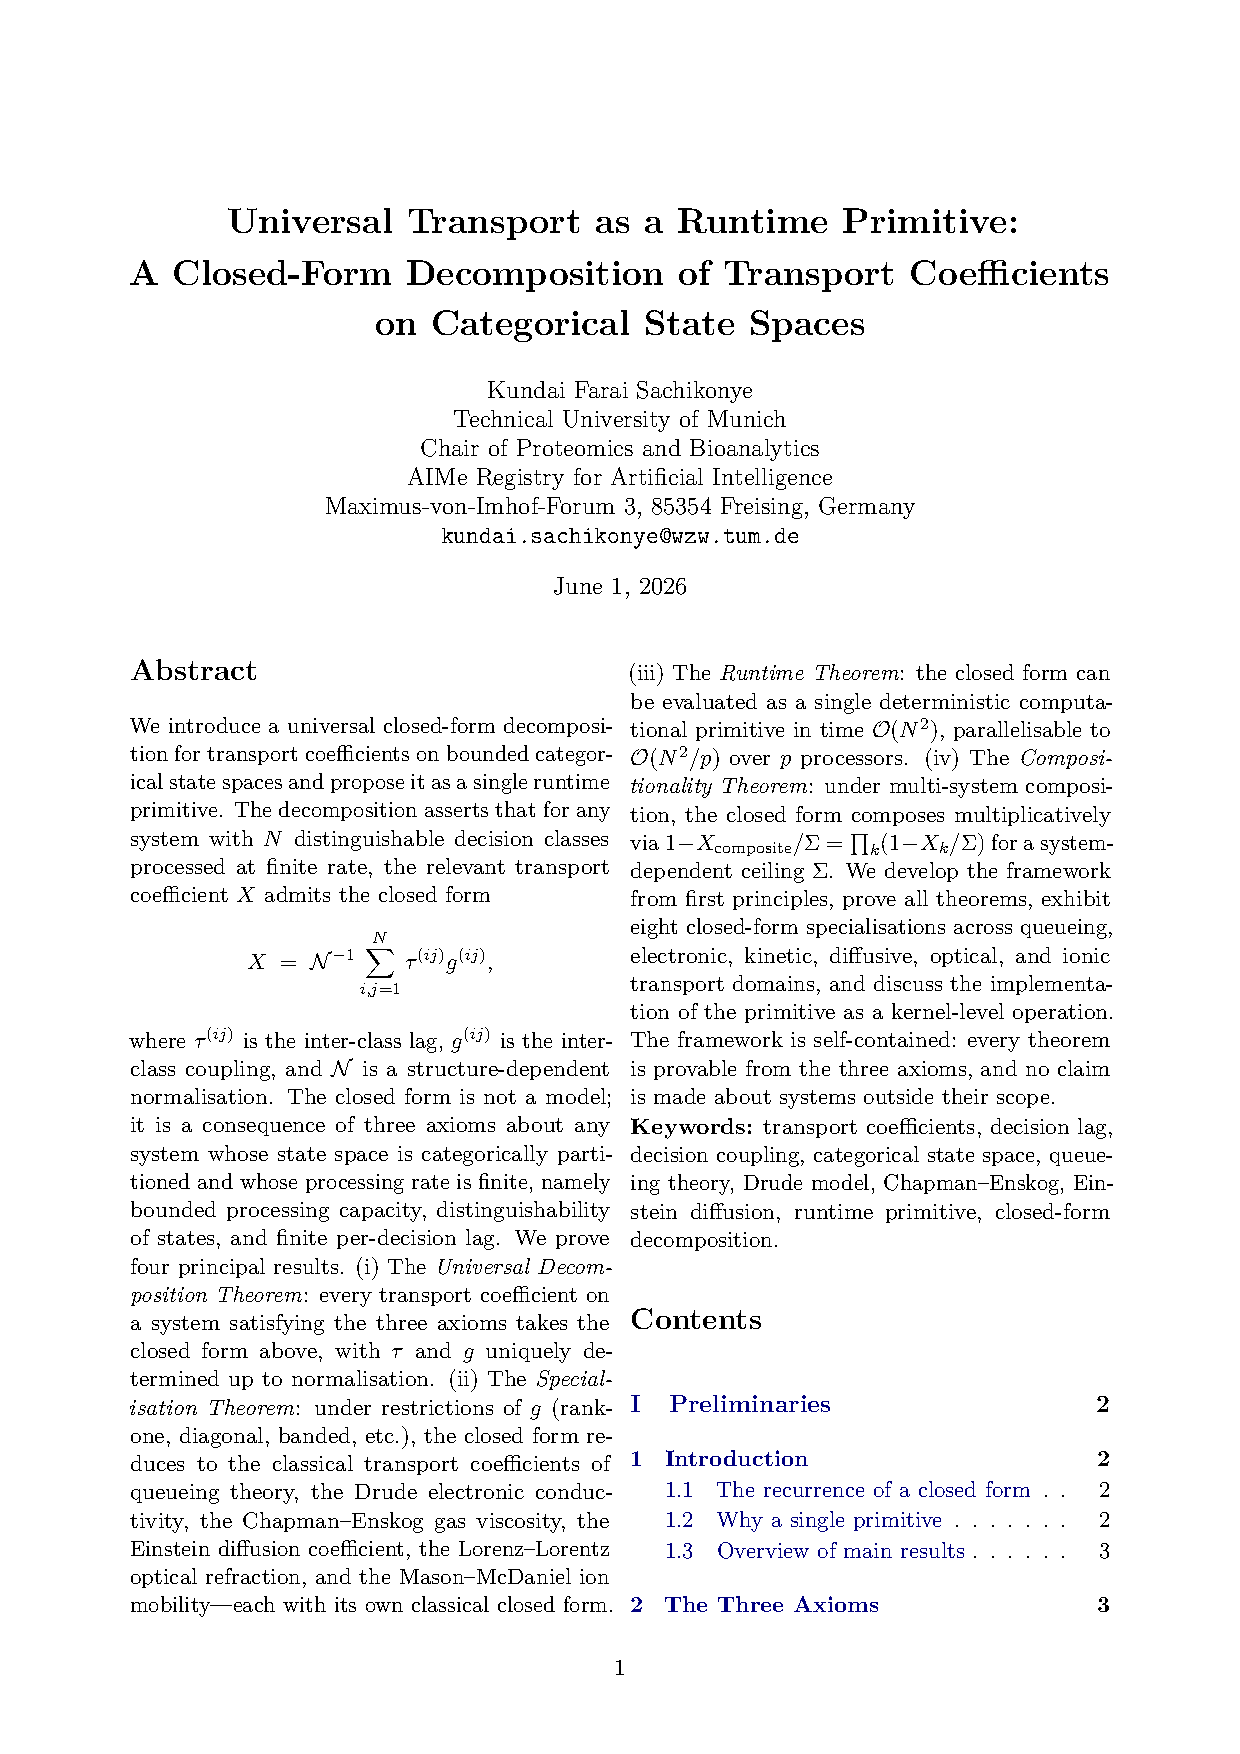
\includepdf[pages=-,
  addtotoc={1, chapter, 1,
    {Paper 14. Universal Transport as a Runtime Primitive:
     A Closed-Form Decomposition of Transport Coefficients
     on Categorical State Spaces},
    paper:transport}
]{operating-system/runtime-primitive/universal-runtime-primitive.pdf}

\phantomsection
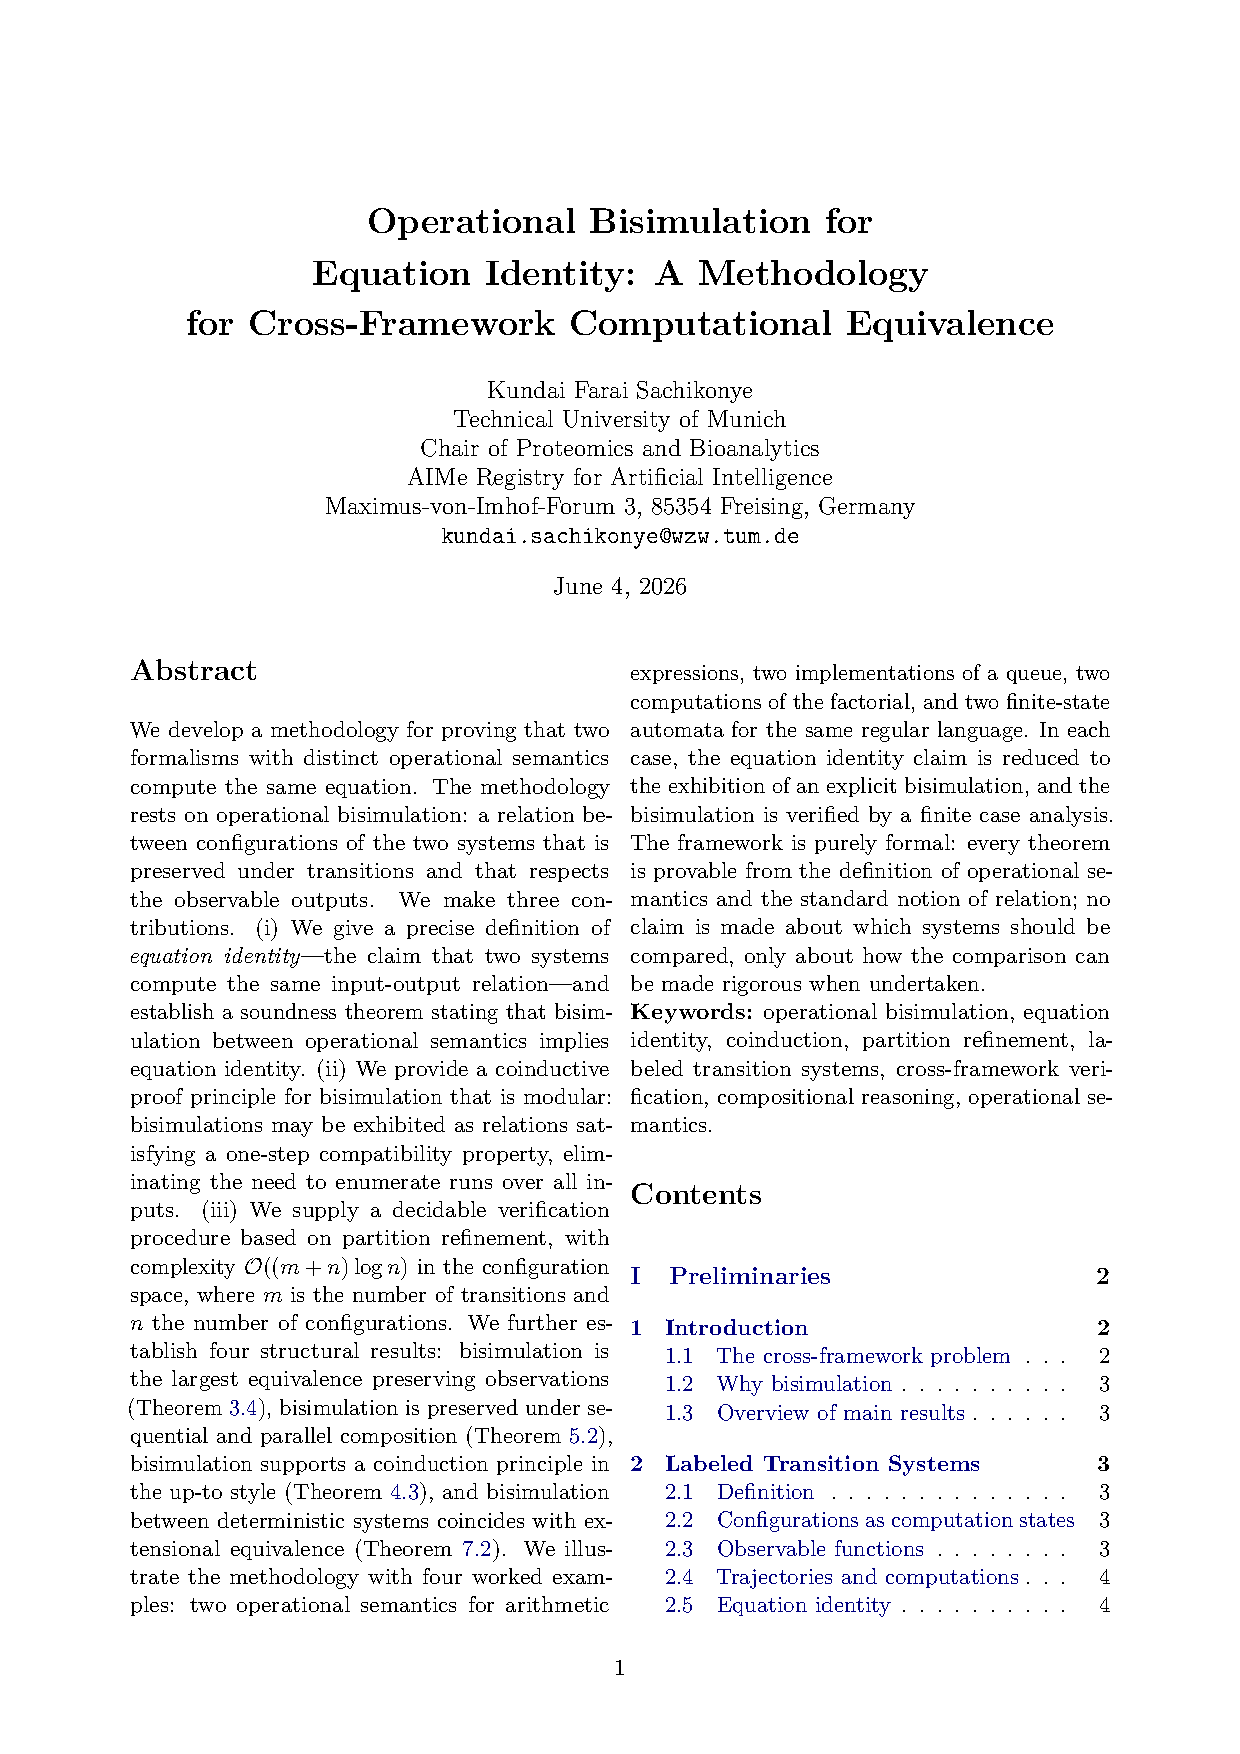
\includepdf[pages=-,
  addtotoc={1, chapter, 1,
    {Paper 15. Operational Bisimulation for Equation Identity:
     A Methodology for Cross-Framework
     Computational Equivalence},
    paper:bisim}
]{operating-system/operational-bisimulation/operational-bisimulation-equation-identity.pdf}

\phantomsection
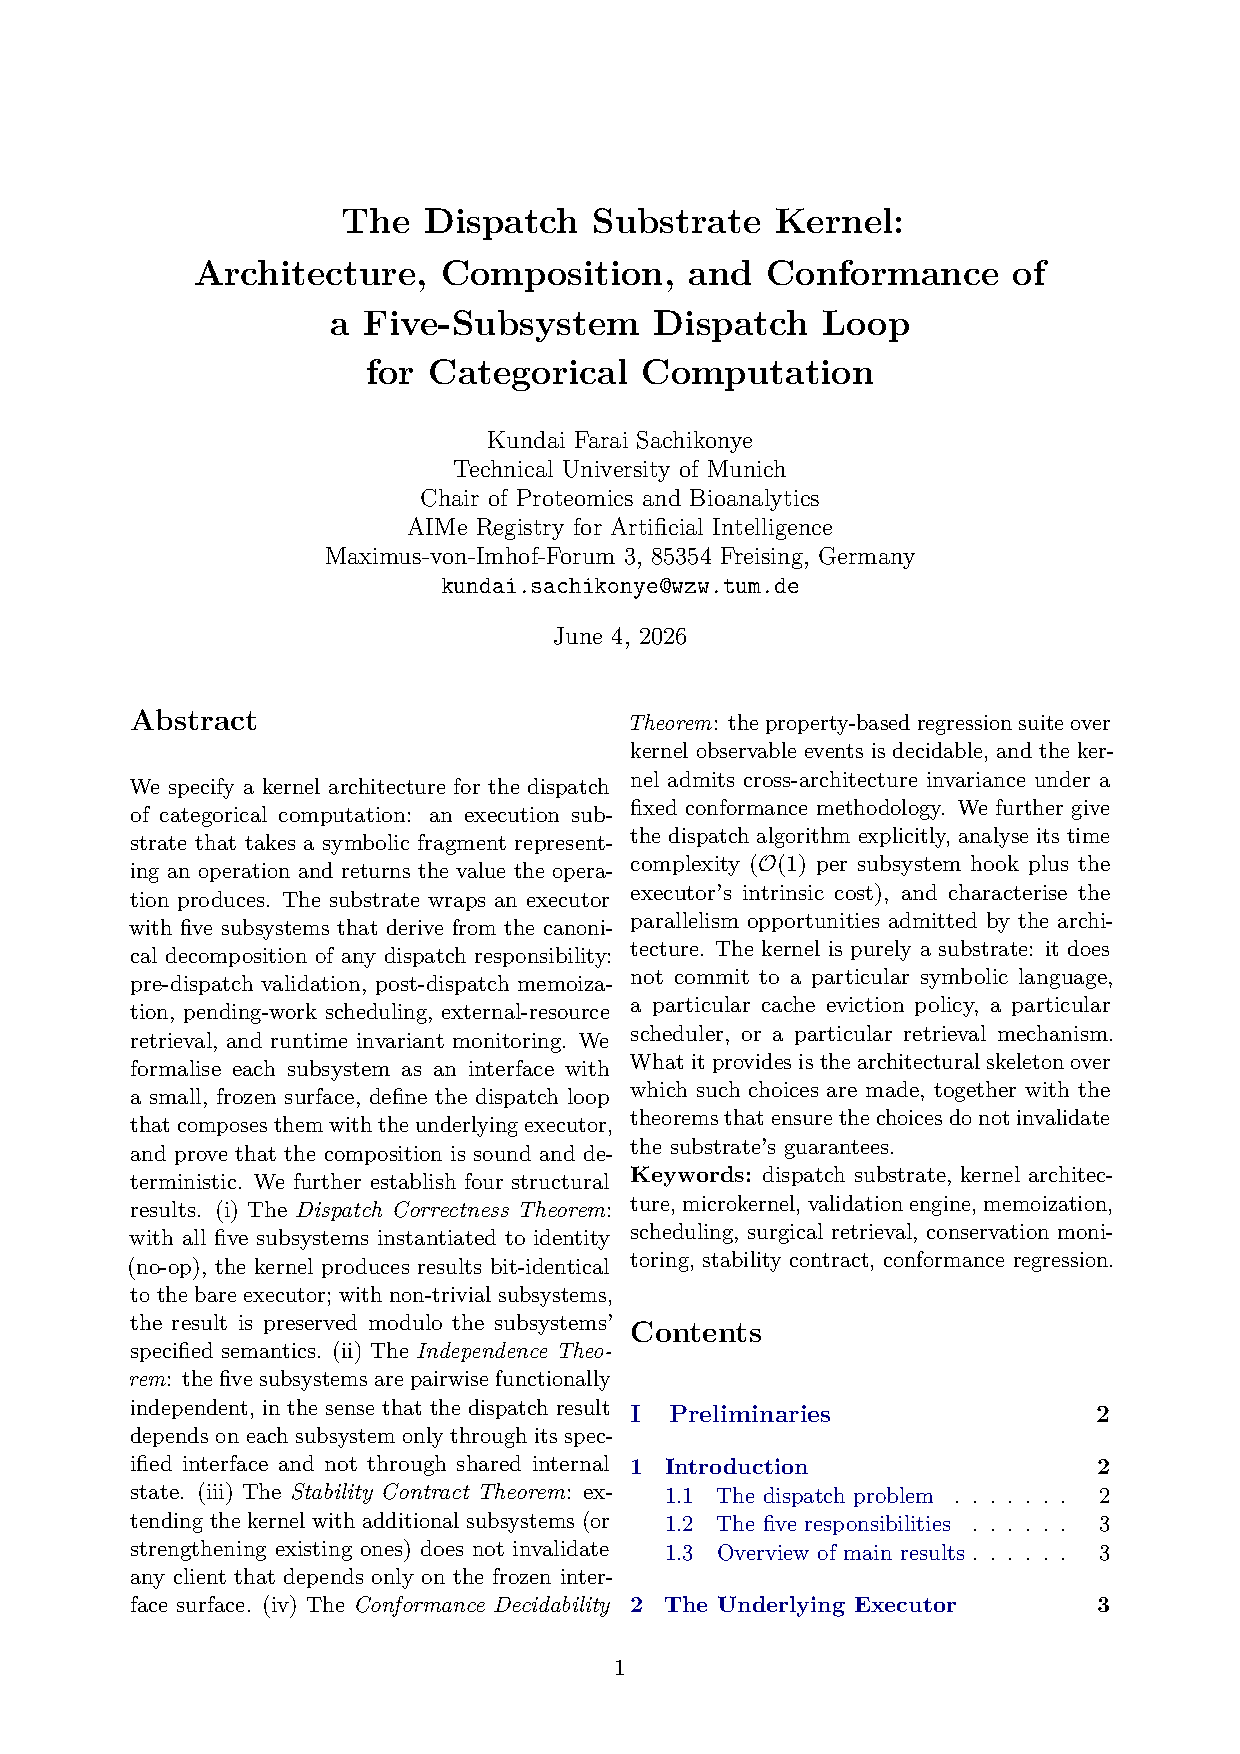
\includepdf[pages=-,
  addtotoc={1, chapter, 1,
    {Paper 16. The Dispatch Substrate Kernel:
     Architecture, Composition, and Conformance of a
     Five-Subsystem Dispatch Loop for Categorical Computation},
    paper:kernel}
]{operating-system/dispath-substrate/dispatch-substrate-kernel.pdf}

% =================================================================
% PART VI — CLOSED LOOP
% =================================================================
\part{Closed Loop}
\label{part:closed_loop}
\addtocontents{toc}{\protect\vspace{1ex}}

\phantomsection
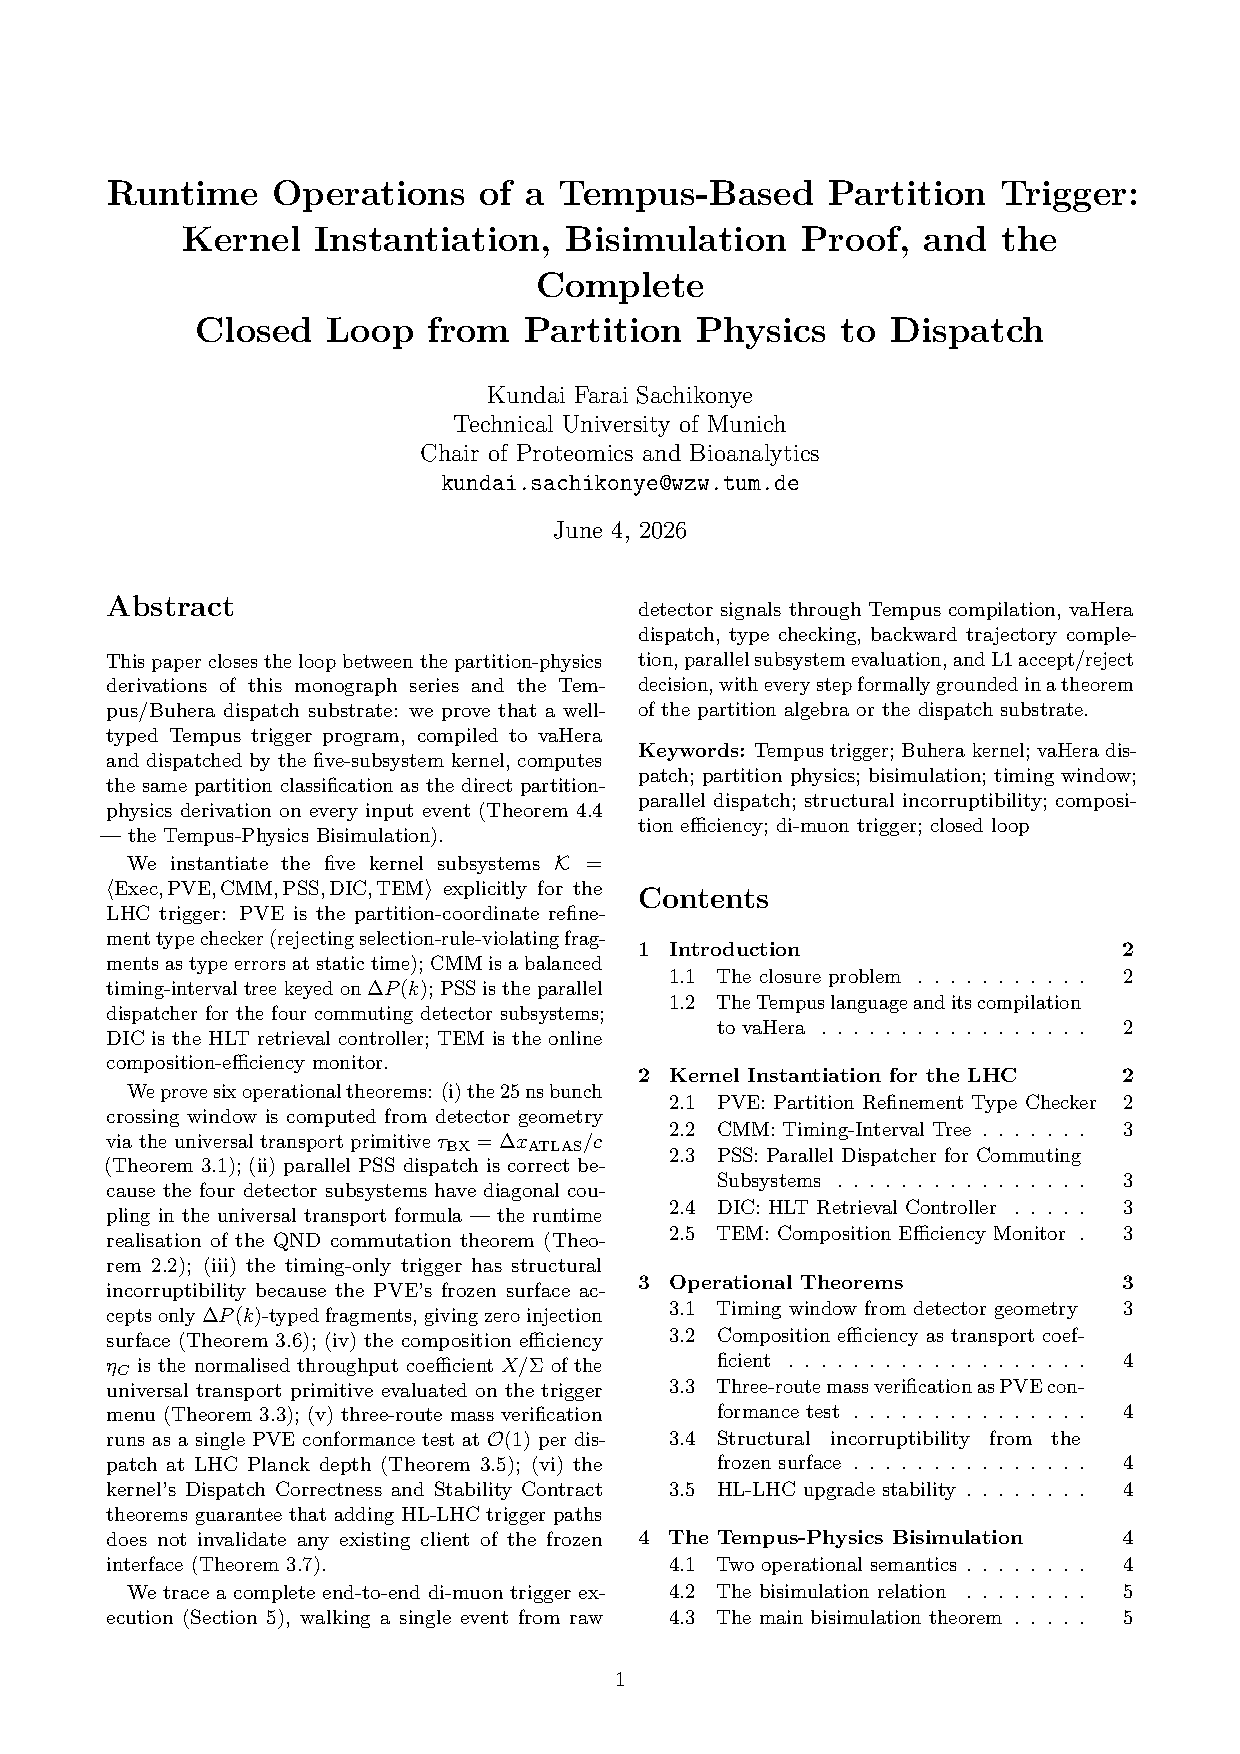
\includepdf[pages=-,
  addtotoc={1, chapter, 1,
    {Paper 17. Runtime Operations of a Tempus-Based Partition Trigger:
     Kernel Instantiation, Bisimulation Proof, and the Complete
     Closed Loop from Partition Physics to Dispatch},
    paper:runtime}
]{runtime-operations/runtime-operations.pdf}

% =================================================================
% PART VII — EXTENSIONS AND CROSS-DOMAIN SYNTHESIS
% =================================================================
\part{Extensions and Cross-Domain Synthesis}
\label{part:extensions}
\addtocontents{toc}{\protect\vspace{1ex}}

\phantomsection
\includepdf[pages=-,
  addtotoc={1, chapter, 1,
    {Paper 18. The Extended Virtual Partition Tensor for
     High-Energy Collisions: Optical Channels, Crossing Symmetry
     as Ritz Combinations, and Bidirectional S-Entropy Reconstruction},
    paper:extensor}
]{extended-partition-tensor/extended-partition-tensor.pdf}

% ------ Back matter -----------------------------------------------
\clearpage
\thispagestyle{empty}
\vspace*{\fill}
\begin{center}
\rule{0.5\textwidth}{0.5pt}\\[1ex]
{\small Derived from the Bounded Phase Space Axiom.\\
Every result in this monograph is a theorem.\\
No free parameter is introduced beyond the caesium-133 calibration constant~$\alpha$.}\\[1ex]
\rule{0.5\textwidth}{0.5pt}
\end{center}
\vspace*{\fill}

\end{document}
